% This is samplepaper.tex, a sample chapter demonstrating the
% LLNCS macro package for Springer Computer Science proceedings;
% Version 2.21 of 2022/01/12
%
\documentclass[runningheads]{llncs}
\usepackage{svg}
\usepackage{amsmath}
\usepackage{graphicx}
\usepackage{hyperref}
\usepackage{color}
\usepackage{tikz}
\usepackage{cite}
\usepackage{booktabs}
\usepackage{float}
\usepackage{amsmath}
\usepackage{amsfonts}
\usepackage{amssymb}
\usepackage{tikz}
\usepackage{dramatist}
\usepackage{pgf-umlsd}
\usetikzlibrary{positioning}
\usepackage{subcaption}
\usepackage{listings}
\usepackage{xcolor}

\newcommand\instruc[1]{\color{blue}[#1]\color{black}}

\begin{document}
%
\title{ {\rm Master Thesis}\\[5pt]Cell\_IA: An intuitive modular framework in Julia for Cellular Automata}
%
%\titlerunning{Abbreviated paper title}
% If the paper title is too long for the running head, you can set
% an abbreviated paper title here
%
\author{
Celia Hermoso Soto\inst{1} \\[15pt]
\small
Supervisor: Enrique Fern\'andez Blanco\inst{2,3} \\
Supervisor: Daniel Rivero Cebri\'an\inst{3}
}
%
\authorrunning{Celia Hermoso Soto}
% First names are abbreviated in the running head.
% If there are more than two authors, 'et al.' is used.
%
\institute{University of A Coru\~na, Spain \\
\email{cel.her.sot@gmail.com}}




%
\maketitle       % typeset the header of the contribution
\tikz [remember picture, overlay] %
\node [shift={(5.3cm,0cm)}] at (current page.north west) %
[anchor=north west] %
{\includegraphics[scale=0.15]{logo.png}};
\tikz [remember picture, overlay]
\node [shift={(6.3cm,0.2cm)}] at (current page.north west) %
[anchor=north west] %
{\includegraphics[scale=0.2]{03_Simbolo_logo_cor.pdf}};
%
\begin{abstract}
La simulación de sistemas complejos constituye una herramienta crucial en diversas disciplinas científicas para comprender dinámicas espaciales y fenómenos emergentes. A pesar de la existencia de herramientas consolidadas, la comunidad investigadora carece de frameworks altamente eficientes que soporten de forma nativa y unificada tanto modelos discretos clásicos, como el Juego de la Vida de Conway, como generalizaciones continuas de alto coste computacional, tales como Lenia. Para abordar esta limitación, este Trabajo de Fin de Máster presenta un framework modular desarrollado en Julia, un lenguaje seleccionado por su rendimiento computacional y su creciente adopción en el ámbito científico. El sistema diseñado permite la ejecución síncrona y asíncrona, soportando diversos tipos de estado de celda y topologías espaciales mediante una arquitectura muy parametrizable. Adicionalmente, con el objetivo de reducir la barrera de entrada técnica, el framework integra un Modelo de Lenguaje Grande (LLM). Esta interfaz interactiva permite a usuarios de diversos perfiles configurar parámetros y generar reglas de evolución mediante instrucciones en lenguaje natural. En pocas palabras, esta herramienta podría proporcionar un entorno de simulación robusto y accesible para usuarios técnicos y no técnicos, acelerando el prototipado de modelos y contribuyendo al avance del estudio de la vida artificial.

\keywords{Autómatas Celulares \and Julia \and Sistemas Complejos \and Modelos de Lenguaje (LLM) \and Juego de la Vida \and Lenia.}
\end{abstract}
%
%
%
\newpage
\pagestyle{empty}
\phantom{a}

\vspace{100pt}
{\bf Enrique Fern\'andez Blanco} and {\bf Daniel Rivero Cebri\'an}, supervisors of the Master Thesis entitled:
\begin{quote}
{\em Cell\_IA: An intuitive modular framework in Julia for Cellular Automata}
\end{quote}
by the student {\bf Celia Hermoso Soto} authorise the submission of this document for the partial fulfillment of the requirements for the degree of Master in Artificial Intelligence, Universidade da Coru\~na.

\vspace{30pt}
A Coru\~na, \instruc{date}


\vspace{80pt}

\begin{tabular}{c@{\hspace{60pt}}c}

Signed: {\bf Enrique Fern\'andez Blanco}
&
Signed: {\bf Daniel Rivero Cebri\'an}
\end{tabular}

\newpage
\section*{Acknowledgements}
\pagestyle{headings}

\newpage
\section{Introducción}
\label{sec:introduccion}
Existe un área de estudio multidisciplinar cuyo objetivo principal es la recreación sintética de fenómenos complejos, frecuentemente inspirados en sistemas biológicos, pero no limitados a ellos, a través de soportes computacionales o físicos; esta disciplina se conoce como Vida Artificial (ALife). La ALife rompe con el enfoque clásico de las ciencias tradicionales, que estudian responder a la pregunta: ``¿Cómo es la realidad''. En su lugar, se atreve a explorar una cuestión más profunda: ``¿Cómo podría ser la realidad?''. En este sentido, la Vida Artificial puede entenderse como un marco amplio para el estudio de sistemas multiagente dinámicos, en los que entidades autónomas, desde celdas en autómatas celulares hasta agentes dotados de modelos más sofisticados, como redes neuronales o modelos de lenguaje, interactúan dando lugar a comportamientos emergentes. Mediante la abstracción de principios organizativos, y su implementación en entornos artificiales a través de modelos estocásticos, sistemas emergentes y algoritmos evolutivos, la Vida Artificial (ALife) permite explorar fenómenos como la complejidad, la autoorganización y la adaptabilidad, proporcionando una perspectiva integradora para comprender los mecanismos fundamentales que rigen tanto sistemas naturales como artificiales desde un punto de vista informacional y funcional.\\

Dentro de este marco concecptual, los Autómatas Celulares (AC) emergen como uno de los formalismos matemáticos y computacionales más robustos para operativizar dicha abstracción. Estructuralmente, se definen como una red regular de celdas, donde cada unidad puede adoptar un estado específico dentro de un conjunto finito de posibilidades. La evolución temporal del sistema se rige por la aplicación de reglas de transición locales, las cuales determinan el estado futuro de una celda en función de su condición actual y la de su vecindad inmediata. A pesar de su aparente simplicidad, debido a sus reglas individuales, los AC son capaces de manifestar comportamientos globales de alta complejidad y patrones emergentes, lo que los convierte en herramientas interesantes para simular procesos dinámicos de la vida real.\\

En este contexto, los ACs \cite{ref_ca}, han permitido a la ciencia moderna explorar procesos que van desde la biología \cite{ref_grow} hasta la sociología \cite{ref_societies, ref_epi} o economía \cite{ref_schelling, ref_economy}. Aunque estos sistemas comparten similitudes con los Modelos Basados en Agentes (ABM) \cite{ref_abm}, los ACs se centran característicamente en dinámicas espaciales discretas sobre cuadrículas, con la intención de recrear los distintos estados que pueden tomar las celdas a lo largo del tiempo, y los ABMs en Agentes, se centran en percibir a los agentes como entidades autónomas que pueden moverse libremente por el entorno, ya sea discreto o continuo. La relevancia de los AC reside en que su aplicación se extiende en áreas muy diversas, como la oncología computacional, donde se utilizan para la evaluación de crecimientos de tumores \cite{ref_tumor}, permitiendo simular cómo las células cancerosas interactúan con su entorno. Asimismo, se han desarrollado enfoques más avanzados orientados al modelado de sistemas celulares artificiales, siendo este conocido como Embriogénesis Artificial \cite{ref_sistema_celular, ref_embryogeny}. Sin embargo, los investigadores a menudo se enfrentan a una limitación: las herramientas existentes suelen obligar a elegir entre facilidad de uso o eficiencia, o la creación y utilización de frameworks muy especializados en atacar la tarea concreta que se plantea\cite{ref_greans}.\\

A pesar del potencial de los ACs para la simulación de sistemas complejos y su creciente avance y aplicación en diversas áreas de conocimiento, la implementación de estos modelos requiere de entornos de programación que logren equilibrar la expresividad matemática con un alto rendimiento computacional. En este sentido, Julia \cite{ref_julia} emerge como una alternativa especialmente atractiva, no solo por su rendimiento, sino también por su ecosistema científico en crecimiento, que incluye librerías avanzadas para computación numérica, simulación y modelado basado en agentes \cite{ref_agentsjl}.\\

Sin embargo, al analizar su ecosistema (reconocido por su capacidad para la computación científica de alto nivel), se observa una carencia significativa en cuanto a librerías o frameworks especializados que faciliten la definición y ejecución optimizada de ACs de propósito general. Esta ausencia de herramientas dedicadas en un lenguaje diseñado específicamente para el rendimiento sugiere una brecha técnica que limita la experimentación, planteando así la necesidad de desarrollar soluciones que integren la flexibilidad de Julia con las exigencias estructurales de los sistemas discretos emergentes. Además, en muchos casos, la comunidad investigadora debe recurrir al uso de múltiples herramientas o lenguajes, lo que introduce complejidad adicional, reduce la reproducibilidad y dificulta la experimentación.

\subsection{Objetivos del proyecto}
Este proyecto nace de la necesidad de proporcionar una herramienta que combine una alta eficiencia de cómputo con una flexibilidad modular y accesible, algo que actualmente no se encuentra de forma integrada en el ecosistema científico. Por tanto, se busca cubrir las necesidades tanto para usuarios no técnicos, gracias a su facilidad de uso e implementación, como para usuarios técnicos, que podrían definir y parametrizar agentes avanzados. Todo ello con el fin de servir a investigadores que necesiten transitar de forma fluida entre modelos complejos; permitiendo definir, implementar y analizar autómatas celulares bajo distintos paradigmas, y facilitando el cambio entre espacios discretos y continuos, así como entre agentes con diferentes estructuras de estado.\\

En este sentido, el objetivo principal de este Trabajo de Fin de Máster es desarrollar, en el lenguaje de programación Julia, un framework que proporcione soporte integral para la implementación y simulación de autómatas celulares, diseñado para incorporar tanto modelos clásicos, como el Juego de la Vida de Conway (GOL) \cite{ref_gol}, como generalizaciones continuas tales como Lenia \cite{ref_lenia}.\\

Para alcanzar el propósito principal, se definen los siguientes objetivos específicos:
\begin{itemize}
    \item \textbf{Eficiencia computacional:} Garantizar un alto rendimiento tanto en modelos discretos como continuos, aprovechando capacidades de computación paralela y multihilo para gestionar grandes volúmenes de datos.
    \item \textbf{Versatibilidad espacial, temporal y multiestado:} Diseñar una estructura de agentes universales (\textit{UniversalAgent}) que permita la definición de múltiples tipos de datos (booleanos, flotantes, strings, enteros, estructuras complejas) y estados internos, facilitando la representación de sistemas heterogéneos. Además de implementar un sistema modular que soporte diversas topologías espaciales (redes cuadradas, hexagonales, espacios continuos y proyecciones 3D) junto con actualizaciones síncronas o asíncronas.
    \item \textbf{Extensibilidad y estandarización:} Proveer un sistema de configuración basado en estándares que permita a los usuarios técnicos extender las funcionalidades del framework sin modifical el núcleo del sistema.
    \item \textbf{Modelado multidisciplinar:} Mostrar la aplicabilidad del framework mediante la implementación de casos de estudio en diversas áreas, desde la biología teórica (GOL o Lenia) hasta la economía sociológica, como el Modelo de Segregación de Schelling (SMS)\cite{ref_schelling}).
    \item \textbf{Interfaz de abstracción mediante LLM:} Desarrollar un módulo generativo (LLMBuilder) que actúe como puente entre el lenguaje natural y el código ejecutable, permitiendo que usuarios sin conocimientos de programación puedan configurar y lanzar simulaciones complejas.
\end{itemize}

En este contexto, el proyecto se concreta en el diseño de una arquitectura flexible y eficiente orientada a la simulación de modelos como Lenia y el Juego de la Vida, incorporando mejoras en la visualización y en los mecanismos de configuración. Todo ello aprovechando el alto rendimiento de Julia para mitigar los cuellos de botella computacionales presentes en otros lenguajes y frameworks.\\

\subsection{Contribuciones principales}
Las contribuciones originales de este trabajo, diseñadas e implementadas, se pueden sintetizar en los siguientes puntos:

\begin{itemize}
    \item \textbf{Framework modular en Julia para ACs:} Diseño e implementación de una arquitectura de cinco módulos desacoplados (\texttt{SpaceDefinition}, \texttt{UniversalAgent}, \texttt{CustomEvolutionRules}, \texttt{Initialization}, \texttt{Representation}) que permite definir y ejecutar simulaciones de autómatas celulares de forma declarativa, sin modificar el núcleo del sistema.
    \item \textbf{Soporte nativo de rejillas hexagonales:} Implementación de un módulo espacial que incluye topología hexagonal con métricas de distancia correctas, cubriendo una carencia explícita del ecosistema actual de Agents.jl y permitiendo simulaciones isotrópicas más fieles a los fenómenos físicos y biológicos.
    \item \textbf{Motor de autómata continuo: Lenia en Julia:} Primera implementación nativa en Julia del modelo Lenia \cite{ref_lenia}, basada en convoluciones eficientes mediante Transformadas Rápidas de Fourier (FFT), integrando espacio continuo, kernel anular y función de crecimiento gaussiana dentro del mismo framework.
    \item \textbf{Interfaz de generación de simulaciones mediante LLM:} Diseño e implementación del módulo \texttt{LLMBuilder}, que utiliza el modelo cuantizado \texttt{qwen2.5-1.5b-coder-q4\_k\_m.gguf} ejecutado localmente junto con una estrategia de \textit{prompt engineering} para traducir descripciones en lenguaje natural a archivos de configuración (\texttt{config.toml}) y código de reglas (\texttt{rules.jl}) ejecutables directamente por el framework.
    \item \textbf{Agente universal multiestado (\texttt{UniversalAgent}):} Diseño de un tipo de agente genérico que permite tipar dinámicamente el estado de la celda como booleano, entero, flotante, símbolo, cadena de texto o estructura personalizada, sin cambios en el núcleo del sistema.
\end{itemize}

El resto de este documento se organiza de la siguiente manera: primero se presenta la Introducción (Sección \ref{sec:introduccion}), luego el Background (Sección \ref{sec:background}), donde se exponen los fundamentos teóricos de los ACs, su evolución histórica, también se analizan los frameworks existentes en la actualidad y se estudia el uso de Julia y Agents.jl. Después de la exposición de la metodología (Sección \ref{sec:metodologia}), se describe detalladamente el trabajo desarrollado (Sección \ref{sec:desarrollo}). Más tarde, se muestra la evaluación y discusión (Sección \ref{sec:evaluacion}) de los resultados. Finalmente, se exponen las conclusiones  del trabajo y el trabajo a futuro (Sección \ref{sec:conclusiones}), y el documento concluye con el apartado de referencias bibliográficas.

%% AAAAAAAAAAAAAAAAAAAAAAAAAAAAAAAAAAAAAAAAAAA
\section{Background}
\label{sec:background}
El estudio de los sistemas complejos mediante simulación computacional se divide tradicionalmente en los Autómatas Celulares (AC) \cite{ref_ca} y los Modelos Basados en Agentes (ABM) \cite{ref_abm}. Mientras que los AC se centran en la evolución de celdas en una rejilla fija, los ABM \cite{ref_abm} permiten una movilidad y autonomía mayor de las entidades. En esta sección se analizarán tanto los modelos teóricos de referencia como las herramientas existentes, con el fin de contextualizar el trabajo aquí desarrollado.

\subsection{Autómatas celulares}
Antes de abordar modelos concretos, es necesario introducir los conceptos básicos que definen un AC. Estos están compuestos por un conjunto de “células” organizadas en un espacio. Entendiéndose por célula, una unidad discreta del sistema que actúa como un agente elemental, caracterizada por un estado interno definido y cuya evolución en el tiempo viene determinada por una función de transición. La evolución del sistema viene determinada por esa función de transición, que en función del estado actual de una célula y el de su vecindario (también definido), define su estado en el siguiente instante temporal.\\

Dependiendo del modelo, tanto espacio como tiempo pueden ser discretos o continuos. En los AC clásicos, el espacio se representa como una rejilla discreta y el tiempo avanza en pasos discretos, mientras que en generalizaciones más recientes, estos elementos pueden tratarse de forma continua.\\

Otro aspecto relevante es el esquema de actualización: en una transición síncrona, todas las células se actualizan simultáneamente en cada paso de tiempo, mientras que en una transición asíncrona, las actualizaciones se realizan de forma secuencial o estocástica. Estos elementos constituyen la base conceptual sobre la que se construyen los modelos que se describen en las siguientes subsecciones.

\subsection{Base matemática de los Autómatas Celulares}
Para comprender un AC, es preciso e interesante desglosarlo en sus componentes algebraicos. Formalmente, un autómata celular se define como una 4-tupla $\mathcal{A} = (\mathcal{L}, S, \mathcal{N}, f)$, cuyos componentes se detallan a continuación para facilitar su comprensión:
\begin{itemize}
    \item \textbf{El espacio de juego ($\mathcal{L}$):} Representa el tablero o rejilla donde ``viven'' las células. Entendiéndose célula como la unidad básica de un sistema, capaz de contener información e interactuar con su entorno. El espacio es, matemáticamente, un conjunto de celdas indexadas por vectores de enteros en $\mathbb{Z}^d$, donde $d$ es la dimensión (por ejemplo, $d=2$ para un tablero plano). Para ello, podría ser práctico imaginar una hoja de papel cuadriculado infinito, donde cada cuadrado es una posición identificable por coordenadas $(x, y)$.
    \item \textbf{El repertorio de estados ($S$):} Es el conjunto de valores que puede adoptar una célula. En el caso más simple, $S = \{0, 1\}$, que podemos interpretar como ``muerto'' o ``vivo''. Si una celda $i$ en el tiempo $t$ tiene el valor $s_i^t = 1$, significa que está activa en ese instante y en ese ``cuadrito''. Este espacio puede ser mucho más complejo, incluyendo valores reales en el intervalo $[0, 1]$ para representar densidades o concentraciones.
    \item \textbf{El vecindario ($\mathcal{N}$):} También conocida como la ``zona de influencia''. Define qué células afectan a una célula concreta. Se describe como un conjunto de desplazamientos relativos $\{v_1, v_2, \dots, v_k\}$, donde $k$ representa el tamaño del vecindario (número de vecinos involucrados) y cada $v_i$ es un vector de $d$ componentes que indica la posición de un vecino respecto a la célula central. Por ejemplo, si el vecindario de una célula incluye a su vecina de la derecha, el vector de desplazamiento sería $v_i = (1, 0)$. Una célula no sabe todo lo que pasa en el tablero, solo puede ``percibir'' lo que ocurre en su vecindario inmediato $\mathcal{N}$.
    \item \textbf{La regla de evolución ($f$):} Es la función de transición local, lo que define qué acción debe tomar la célula. Formalmente, se define como una función $f: S^k \to S$ que recibe los estados actuales de las $k$ celdas que conforman el vecindario y devuelve el nuevo estado que tendrá la célula central en el siguiente instante: $s_i^{t+1} = f(s_{i+v_1}^t, s_{i+v_2}^t, \dots, s_{i+v_k}^t)$.
\end{itemize}

Esta formulación matemática garantiza dos principios críticos: la homogeneidad (la regla $f$ es la misma para todos, sin importar la posición en el espacio) y la localidad (el cambio solo depende de lo que ocurre cerca), permitiendo que la autoorganización emerja sin necesidad de un control centralizado.

\subsection{Modelos Basados en Agentes (ABM)}
Si bien los ACs permiten modelar sistemas complejos mediante reglas locales en una rejilla estática, los ABMs expanden este paradigma al centrar la atención en la entidad individual (el agente) más que en el espacio que ocupa.\\

Aunque comparten la filosofía de la descentralización y la emergencia de patrones globales a partir de reglas locales, los ABM introducen diferencias fundamentales respecto a los AC:
\begin{itemize}
    \item \textbf{Movilidad:} A diferencia de las células en un AC, que están ancladas a una posición fija en la rejilla, los agentes en un ABM suelen tener la capacidad de desplazarse por un espacio que puede ser discreto o continuo.
    \item \textbf{Heterogeneidad:} Mientras que los AC son intrínsecamente homogéneos (todas las células siguen la misma regla $f$), en un ABM cada agente puede poseer estados internos únicos, objetivos distintos o incluso reglas de comportamiento diferenciadas.
    \item \textbf{Interacción:} En los ABM, las interacciones no están limitadas exclusivamente a la topología de una rejilla; los agentes pueden interactuar por proximidad física, pero también a través de redes sociales, intercambio de mensajes o manipulación de un entorno compartido (llamado estigmergia).
\end{itemize}
En esencia, se puede considerar a los ACs como un caso particular de ABMs donde los agentes son estáticos, idénticos y están dispuestos en una red regular. No obstante, la distinción es necesaria para abordar sistemas donde la individualidad y el movimiento son los motores principales de la dinámica del modelo.

\subsection{Componentes estructurales y tipologías}
La arquitectura de un sistema basado en agentes o células determina cómo fluye la información y qué tipo de patrones pueden formarse.

\subsubsection{Topologías de rejilla}
La disposición de las celdas condiciona la simetría del sistema. Las variaciones en la rejilla $\mathcal{L}$ alteran la conectividad:
\begin{itemize}
    \item \textbf{Rejilla cuadrangular:} Es el estándar por su facilidad de implementación en matrices de datos. Sin embargo, presenta el inconveniente de que las distancias a los vecinos no son uniformes si se quieren aplicar métricas para la distancia, ya que los vecinos en diagonal están más lejos que los ortogonales.
    \item \textbf{Rejilla hexagonal:} Es altamente valorada en simulaciones científicas porque ofrece isotropía, es decir, la ausencia de direcciones ``privilegiadas'' en la interacción entre celdas. Esta propiedad evita sesgos direccionales presentes en otras discretizaciones y la hace especialmente adecuada para modelar fenómenos físicos continuos, como fluidos o tejidos biológicos \cite{ref_wolfram, ref_lattice_gas}. En este caso, cada célula tiene 6 vecinos a la misma distancia exacta.
    \item \textbf{Rejilla triangular:} Utilizada principalmente en estudios teóricos de redes cristalinas \cite{ref_triangular, ref_triautomata} debido a su rigidez geométrica.
\end{itemize}

\subsubsection{Configuraciones de vecindario}
La definición de $\mathcal{N}$ es uno de los factores que más influye en el dinamismo del sistema. Aunque las definiciones clásicas de vecindario suelen referirse a rejillas cuadrangulares, estas establecen la base para entender el alcance de la interacción; los radios de vecindario $r$ son determinan este alcance. Los modelos avanzados introducen el concepto de ponderación mediane el uso de kernels ($K$). En este enfoque, cada vecino aporta una intensidad específica al cálculo del nuevo estado. Las configuraciones más habituales, y las que se han integrado en el framework, son:
\begin{itemize}
    \item \textbf{Vecindario de Von Neumann:} En su forma estándar para rejillas cuadrangulares, incluye solo a los vecinos que comparten un lado (Norte, Sur, Este, Oeste). Es un entorno de 4 vecinos (o 5 si se cuenta la propia celda).  El kernel asociado sería una matriz donde solo las posiciones ortogonales tienen peso:
    \begin{equation}
    K_{\text{Neumann}} = \begin{pmatrix} 0 & 1 & 0 \\ 1 & 0 & 1 \\ 0 & 1 & 0 \end{pmatrix}
    \end{equation}
    \item \textbf{Vecindario de Moore:} Incluye tanto vecinos ortogonales como diagonales. En una rejilla cuadrada, esto suma 8 vecinos (o 9 si se cuenta la propia celda). Este vecindario se suele tratar de forma uniforme (todos los vecinos tienen peso 1), lo equivalente a un kernel de unos:
    \begin{equation}
    K_{\text{Moore}} = \begin{pmatrix} 1 & 1 & 1 \\ 1 & 0 & 1 \\ 1 & 1 & 1 \end{pmatrix}
    \end{equation}

    Es el estándar en modelos muy extendidos como el Juego de la Vida \cite{ref_gol}.
    \item \textbf{Vecindarios extensos:} En modelos modernos, el radio $r$ puede ser mayor a 1, permitiendo que una célula se vea influenciada por celdas situadas a gran distancia. Estos vecindarios pueden aplicarse tanto a estructuras cuadrangulares como a espacios continuos.
     También suele modelarse mediante kernels de convolución.
\end{itemize}

\begin{figure}[H]
\centering
\begin{subfigure}[b]{0.30\textwidth}
    \centering
    \includegraphics[width=0.8\textwidth]{neumann.png}
    \caption{Von Neumann.}
    \label{fig:neumann}
\end{subfigure}
\hfill
\begin{subfigure}[b]{0.28\textwidth}
    \centering
    \includegraphics[width=0.8\textwidth]{moore.png}
    \caption{Moore.}
    \label{fig:moore}
\end{subfigure}
\hfill
\begin{subfigure}[b]{0.30\textwidth}
    \centering
    \includegraphics[width=0.8\textwidth]{extendido.png}
    \caption{Von Neumann extendido ($r$=2).}
    \label{fig:extendido}
\end{subfigure}
\caption{Ejemplos de configuraciones de vecindario.}
\label{fig:vecindarios}
\end{figure}

\begin{itemize}
     \item \textbf{Kernel Gaussiano:} Siguiendo en la línea de los vecindarios extensos, un kernel Gaussiano es la representación de la influencia degradada con la distancia. A diferencia de los vecindarios binarios, este asigna un peso máximo a la celda central que decae de forma exponencial hacia los extremos según la distribución normal. Una aproximación discreta cómun para una matriz de $5 \times 5$ es:
     \begin{equation}
    K_{\text{Gauss}} = \frac{1}{256} \begin{pmatrix} 
    1 & 4 & 6 & 4 & 1 \\ 
    4 & 16 & 24 & 16 & 4 \\ 
    6 & 24 & 36 & 24 & 6 \\ 
    4 & 16 & 24 & 16 & 4 \\ 
    1 & 4 & 6 & 4 & 1 
    \end{pmatrix}
    \end{equation}

    Este tipo de ponderación suele ser usada para permitir que los patrones emerjan con formas orgánicas y fluidas.
     \item \textbf{Kernels anulares:} Para autómatas continuos como Lenia, a veces se utilizan kernels que definan una ``zona de interés'' en forma de anillo. Estos se representan mediante matrices donde los pesos siguen una distribución radial $K(r)$. Esto es fundamental para lograr que la ``célula'' se comporte igual sin importar en qué dirección se mueva sobre el espacio continuo.
     
\end{itemize}

Como se puede observar, el uso de matrices de pesos transforma la actualización del sistema en una operación de convolución discreta.

\subsubsection{Condiciones de contorno y topologías de frontera}En el plano teórico, muchos modelos de autómatas celulares se conciben sobre rejillas infinitas ($\mathbb{Z}^d$). No obstante, la traslación de estos modelos al dominio computacional impone la restricción de trabajar con dominios finitos debido a las limitaciones de memoria y capacidad de procesamiento. Esta finitud introduce discontinuidades en los extremos de la rejilla que deben resolverse mediante la definición de condiciones de contorno. Las configuraciones más habituales integradas en este framework son:
\begin{itemize}
    \item \textbf{Condiciones periódicas (Topología Toroidal):} Representan la solución más común para evitar el ``efecto borde''. Matemáticamente, el espacio se trata mediante aritmética modular, donde una celda en la posición $(x, y)$ tiene como vecina a la derecha a la celda en $(0, y)$ si $x$ alcanza el límite máximo $L$. Esta configuración proyecta la rejilla plana sobre la superficie de un toroide, eliminando las fronteras físicas y permitiendo que la masa, la energía o los agentes fluyan indefinidamente sin abandonar el sistema. Es la opción preferente para estudiar estados estacionarios y dinámicas de equilibrio.
    \item \textbf{Condiciones fijas o de Valor Constante (Dirichlet):} En este esquema, se define un ``halo'' de celdas virtuales (denominadas \textit{ghost cells}) que rodean el dominio activo y mantienen un estado inmutable $s_{\text{border}} = c$. Es habitual establecer $c=0$ para representar el vacío o la ausencia de recursos. En modelos de propagación de incendios o fluidos, estas fronteras actúan como sumideros o muros infranqueables que absorben cualquier dinámica que entre en contacto con ellas.
    \item \textbf{Condiciones reflectantes (Especulares):} El borde actúa como un espejo simétrico. Cuando una regla de transición consulta un vecino más allá del límite, el sistema devuelve el valor de la celda interna simétricamente opuesta. Este modelo es esencial en la simulación de dinámica de ondas o acústica, ya que permite que los frentes de onda reboten en las paredes del dominio conservando su energía, lo que resulta fundamental para observar fenómenos de interferencia y resonancia dentro de un recinto cerrado.
    \item \textbf{Condiciones adiabáticas o de Flujo Nulo (Neumann):} A diferencia de las condiciones de Dirichlet, aquí el valor del borde no es una constante externa, sino que se iguala dinámicamente al valor de la celda adyacente interna: $s_{\text{borde}} = s_{\text{interno}}$. Esto garantiza que el gradiente en la frontera sea cero ($\nabla s = 0$), lo cual es indispensable en simulaciones de procesos de difusión térmica o química donde no debe haber intercambio de flujo con el exterior del sistema.
    \item \textbf{Condiciones helicoidales:} Una variante de las periódicas utilizada frecuentemente para mapear autómatas bidimensionales en vectores unidimensionales de alto rendimiento. Al llegar al final de una fila, la conexión se realiza con el inicio de la fila siguiente con un desplazamiento de una unidad. Aunque su interpretación física es menos intuitiva, ofrece ventajas computacionales en el acceso a memoria lineal.
\end{itemize}

\subsection{Evolución histórica y modelos de referencia}
La génesis de los Autómatas Celulares (AC) no responde únicamente a una curiosidad matemática, sino a una búsqueda fundamental por comprender la naturaleza de la autoorganización y la computación universal en sistemas biológicos y físicos. Históricamente, el desarrollo de los AC representa una ruptura con el paradigma reduccionista, proponiendo en su lugar que la complejidad de un sistema no reside en la sofisticación de sus componentes individuales, sino en la riqueza de sus interacciones locales: la emergencia.\\

Para comprender el alcance de este TFM, es imperativo analizar la trayectoria de estos modelos, los cuales han transitado desde la discreción de los estados binarios hacia la fluidez de los sistemas continuos. A continuación, se examinan los hitos y modelos de referencia que han configurado este dominio: partiendo de la arquitectura fundacional de Von Neumann, pasando por la explosión de complejidad del Game of Life de Conway y la sistematización de Wolfram, hasta alcanzar las dinámicas sociales de Schelling y la sofisticación orgánica de Lenia \cite{ref_lenia}.

\subsubsection{Los orígenes: Von Neumann y la autorreplicación}
En los años 40, John von Neumann, influenciado por Stanislaw Ulam, buscaba un marco para la vida artificial. Diseñó el Constructor Universal de Von Neumann \cite{ref_mcmullin_vonneumann} un AC con 29 estados posibles por celda. Su importancia real radica en que demostró que una máquina puramente lógica podía contener las instrucciones para crear una copia de sí misma, anticipándose al descubrimiento de la estructura del ADN.\\

El modelo original se basaba en una rejilla bidimensional donde cada celda podía adoptar uno de 29 estados posibles. Las reglas de transición eran deterministas y estaban diseñadas para simular la lógica de una cinta de computación y un brazo constructor.

\subsubsection{El Juego de la Vida}
El referente fundacional en este campo es el Juego de la Vida (GoL \cite{ref_gol}). Se define como un autómata celular discreto donde cada célula posée un estado binario y evoluciona en pasos de tiempo discretos siguiendo reglas deterministas basadas en el número de vecinos activos. Ver Fig.\ref{fig:gol}. Puede conceptualizarse como un AC, dado que cada célula actúa como un agente local sin aprendizaje, regido exclusivamente por reglas fijas.

Introducido por John Conway en 1970, el \textit{Game of Life} (GoL) \cite{ref_gol} es uno de los modelos de referencia de este proyecto. Como se ha mencionado, se define sobre una rejilla cuadrada bidimensional con estados $S = \{0, 1\}$.
\begin{itemize}
    \item \textbf{Entorno y Agentes:} Las células actúan como agentes binarios en un entorno de Moore ($r=1$).
    \item \textbf{Dinámica Matemática:} Sea $N$ la suma de los estados de los 8 vecinos. La función de transición $f$ se define:
    \begin{enumerate}
        \item \textbf{Supervivencia:} Si $s_i^t=1$ y $N \in \{2, 3\}$, entonces $s_i^{t+1}=1$. Es decir, si de los 8 vecinos de una célula viva, hay 2 o 3 que están vivos, entonces la célula sobrevive.
        \item \textbf{Nacimiento:} Si $s_i^t=0$ y $N = 3$, entonces $s_i^{t+1}=1$. En otras palabras: si alrededor de una célula que está muerta hay exactamente 3 vecinos que están vivos, entonces la célula nace o revive.
        \item \textbf{Muerte:} En cualquier otro caso, $s_i^{t+1}=0$ (la célula muere por soledad si $N<2$ o por sobrepoblación si $N>3$).
    \end{enumerate}
    \item \textbf{Importancia:} GoL es Turing-completo, lo que significa que se puede construir una computadora entera dentro del juego \cite{ref_gol}. Es el ejemplo máximo de cómo reglas simples generan estructuras persistentes (``gliders'', ``pulsars'').
\end{itemize}

\begin{figure}[H]
\centering
\begin{subfigure}[b]{0.48\textwidth}
    \centering
    \includegraphics[width=\textwidth]{gol50.png}
    \caption{Rejilla 50×50.}
    \label{fig:gol}
\end{subfigure}
\hfill
\begin{subfigure}[b]{0.48\textwidth}
    \centering
    \includegraphics[width=\textwidth]{gol512.png}
    \caption{Rejilla 512×512.}
    \label{fig:gol512}
\end{subfigure}
\caption{Ejemplo de simulación del modelo Game Of Life en el framework Cell\_IA.}
\label{fig:gol_combined}
\end{figure}

Las configuraciones experimentales típicas para GoL, emplean rejillas cuadradas con fronteras periódicas (toroidales), variando en tamaño desde 50 x 50 (Ver Fig.\ref{fig:gol}) para experimentos teóricos, hasta 512 x 512 (Ver Fig.\ref{fig:gol512}) para pruebas de rendimiento.\\

Este modelo ha sido ampliamente estudiado debido a su capacidad de generar comportamientos emergentes complejos a partir de reglas muy sencillas, como estructuras estables, osciladores o patrones móviles (gliders), lo que lo convierte en un banco de pruebas ideal para frameworks.

\subsubsection{Stephen Wolfram y la sistematización elemental}
En los 80, Wolfram analizó de forma exhaustiva los AC unidimensionales (una sola línea de celdas), centrándose en aquellos con dos estados posibles y un vecindario de radio $r=1$. Bajo estas restricciones, existen $2^{2^3} = 256$ reglas de evolución posibles, las cuales Wolfram numeró y sistematizó. A pesar de su extrema sencillez, clasificó su comportamiento en cuatro clases, desde la estabilidad total hasta el caos \cite{ref_wolfram}. Entre este catálogo, destacan la Regla 30, generadora de aleatoriedad, y la Regla 110, cuya dinámica es capaz de soportar la computación universal.

\begin{figure}[H]
    \centering
        \begin{subfigure}[b]{0.45\textwidth}
        \centering
        \includegraphics[width=0.6\textwidth]{regla30.png}
        \caption{Evolución de la Regla 30, mostrando su característico patrón caótico y asimétrico. 
        Fuente: Zhiming Wang, licencia CC0 1.0.}
        \label{fig:regla30}
    \end{subfigure}
    \hfill
        \begin{subfigure}[b]{0.5\textwidth}
        \centering
        \includegraphics[width=0.6\textwidth]{regla110.png}
        \caption{Evolución de la Regla 110, donde se aprecian estructuras localizadas (gliders) interactuando. 
        Fuente: LucasVB, \textit{Wikimedia Commons}, licencia CC BY-SA.}
        \label{fig:regla110}
    \end{subfigure}
\end{figure}

\begin{itemize}
    \item \textbf{Clasificación de Wolfram:} Propuso cuatro clases de comportamiento basándose en el destino a largo plazo de la configuración: desde la convergencia a estados homogéneos (Clase I) o estructuras periódicas (Clase II), hasta el comportamiento caótico (Clase III, como la Regla 30) y la complejidad emergente con capacidad de computación universal (Clase IV, donde se sitúa la Regla 110).
    \item \textbf{Aplicación práctica:} Sus trabajos sobre la Regla 30 han sido fundamentales para la generación de números pseudoaleatorios en criptografía \cite{ref_wolfram_crypto}, basándose en la naturaleza caótica y la sensibilidad a las condiciones iniciales de las reglas locales, lo que dificulta la predicción de estados futuros sin computar cada paso intermedio.
\end{itemize}

\subsubsection{Modelos Sociales: El Modelo de Segregación de Schelling}
El modelo de segregación de Schelling \cite{ref_schelling} representa la primera gran aplicación de los AC al comportamiento humano. A diferencia de los modelos físicos o biológicos, aquí las celdas representan hogares en una ciudad.

\begin{itemize}
\item \textbf{Reglas de Agente:} Los agentes poseen un umbral de tolerancia: si el porcentaje de vecinos diferentes a ellos supera un límite, deciden mudarse a una celda vacía.
\item \textbf{Importancia social:} Este modelo demostró que fenómenos macroscópicos indeseados, como la segregación racial urbana, pueden emerger incluso si los individuos no poseen prejuicios extremos, sino simplemente una ligera preferencia por la similitud. Es un puente fundamental entre los AC y los Modelos Basados en Agentes (ABM).
\end{itemize}

\subsubsection{Lenia}
Finalmente, Lenia \cite{ref_lenia} marca la evolución contemporánea de los AC al eliminar la restricción de la discreción. Al operar en un espacio de estados $[0, 1]$ y utilizar funciones de crecimiento continuas, Lenia permite observar una ``biología digital'' mucho más plástica.

\begin{figure}[H]
\centering
\includegraphics[width=0.4\textwidth]{lenia.jpg}
\caption{Ejemplo de simulación del modelo Lenia.
Fuente: Bert Chan, \textit{Lenia Expanded}, 2020.}
\label{fig:lenia}
\end{figure}

\begin{itemize}
    \item \textbf{Kernel y Convolución:} En lugar de reglas lógicas booleanas, utiliza integrales de convolución que permiten una suavidad espacial y temporal. El estado $A$ es continuo $A \in [0, 1]$. La actualización sigue la ecuación:
    \begin{equation}A^{t+\Delta t} = \text{clip}\left( A^t + \Delta t \cdot G(A^t \circledast K) \right)\end{equation}
    Aquí, $\circledast$ representa la operación de convolución, donde un núcleo $K$ (kernel) ``escanea'' la rejilla calculando un promedio ponderado de los estados vecinos.
    
    \item \textbf{Función de truncamiento (\textit{clip}):} El operador $\text{clip}(x)$ es una función de saturación definida como $[x]_0^1 = \max(0, \min(1, x))$. Su propósito es garantizar la estabilidad numérica del sistema, forzando a que los valores de los estados se mantengan estrictamente dentro del intervalo físico $[0, 1]$, evitando que la acumulación de incrementos $\Delta t$ produzca valores divergentes.

    \item \textbf{Función de crecimiento ($G$):} Determina la dinámica del sistema basándose en el nivel de ``activación'' local $u = A \circledast K$. Aunque la forma más común es una campana de Gauss centrada en una media $\mu$ con desviación $\sigma$ ($G(u) = 2 \exp(- \frac{(u-\mu)^2}{2\sigma^2}) - 1$), el modelo permite cualquier función de mapeo. Estas pueden ser multimodales (mezclas de varias gaussianas), funciones escalonadas (para emular comportamientos discretos tipo Juego de la Vida) o funciones polinómicas, permitiendo definir diferentes ``leyes físicas'' para cada simulación.
    
    \item \textbf{Importancia:} Lenia permite la existencia de ``especies'' con metabolismo y movimiento suave, siendo la base para la investigación en vida artificial (ALife) de alto rendimiento. Requiere el uso de Transformadas Rápidas de Fourier (FFT) para realizar las convoluciones de forma eficiente en términos computacionales.
\end{itemize}


\subsection{Análisis comparativo de frameworks de simulación}
En la actualidad, la comunidad científica utiliza diversas herramientas para la simulación de ABM y AC, cada una con compromisos específicos entre usabilidad y rendimiento. Para situar este proyecto, es necesario comparar las soluciones existentes. Cabe destacar que la mayoría de estas no son nativas de Julia, lo que supone una barrera de rendimiento o integración. La tabla \ref{tab:comparativa_frameworks} resume esta comparativa:

\begin{itemize}
    \item \textbf{NetLogo \cite{ref_netlogo}:} Herramienta de una popularidad significativa tanto en la docencia, como el prototipado, debido a su lenguaje sencillo y GUI integrada para visualización en tiempo real. No obstante, presenta limitaciones significativas en rendimiento y escalabilidad para simulaciones complejas.
    \item \textbf{Mesa (Python) \cite{ref_mesa}:} Un framework flexible que soporta rejillas y espacios continuos con visualización web. Su principal ventaja es el ecosistema de Python, pero su eficiencia computacional es inferior a la de lenguajes compilados o Julia.
    \item \textbf{MASON (Java) \cite{ref_mason}:} Ofrece un rendimiento alto y es robusto para la investigación académica, pero carece de una interfaz visual atractiva por defecto y posee una curva de aprendizaje pronunciada.
    \item \textbf{PettingZoo \cite{ref_pettingzoo} y RLib (Python) \cite{ref_rlib}:} Orientados específicamente a entornos de MARL y aprendizaje por refuerzo. Aunque son potentes para investiación en IA, pueden resultar complejos de configurar y no siempre están optimizados para escalas masivas de agentes simples tipo AC.
    \item  \textbf{Agents.jl (Julia) \cite{ref_agentsjl}:} Orientado a agentes, ofrece alto rendimiento e integración con Julia. Soporta espacios discretosy continuos. Sin embargo, requiere conocimientos técnicos para su uso y carece de abstracciones específicas para simulaciones.
\end{itemize}

\begin{table}[h]
\centering
\caption{Comparativa de frameworks de simulación. Se han definido cuatro criterios de evaluación: Eficiencia (E), Flexibilidad de Reglas (F), Facilidad de Uso (U) y Soporte Nativo Julia (J). }
\label{tab:comparativa_frameworks}
\begin{tabular}{@{}lcccc@{}}
\toprule
\textbf{Framework} & \textbf{E} & \textbf{F} & \textbf{U} & \textbf{J} \\ \midrule
NetLogo \cite{ref_netlogo} & Media & Alta & Muy Alta & No \\
Mesa (Python) \cite{ref_mesa} & Baja & Alta & Alta & No \\
MASON (Java) \cite{ref_mason} & Alta & Media & Baja & No \\
Agents.jl \cite{ref_agentsjl} & Alta & Alta & Media & Sí \\
\textbf{Cell\_IA (Propuesto)} & \textbf{Alta} & \textbf{Alta} & \textbf{Muy Alta} & \textbf{Sí} \\ \bottomrule
\end{tabular}
\end{table}

A partir de la Tabla \ref{tab:comparativa_frameworks} se observa que no existe una solución que combine simultáneamente alta eficiencia, facilidad de uso y soporte nativo en Julia. En particular, los frameworks más accesibles presentan limitaciones de rendimiento, mientras que aquellos más eficientes requieren de un mayor esfuerzo de implementación. Esto justifica la necesidad de una propuesta como Cell\_IA, que busca equilibrar estos factores.

\subsection{El ecosistema en Julia: Agents.jl}
La elección de Julia no es trivial: este lenguaje combina la facilidad de uso de lenguajes dinámicos con un rendimiento comparable al de C \cite{ref_julia}, lo cual es crítico en simulaciones que requiren un alto coste computacional. Además, Julia cuenta con una comunidad científica en constante crecimiento que demanda herramientas de simulación de alto rendimiento. Aunque existen herramientas consolidadas en el ecosistema científico, se detecta una carencia de implementaciones nativas en Julia para autómatas continuos como Lenia:

\begin{itemize}
    \item \textbf{Fragmentación: } Herramientas como NetLogo \cite{ref_netlogo} o Mesa \cite{ref_mesa} son excelentes para modelos discretos y agentes, pero sufren mucho en rendimiento cuando se trata de modelos continuos que requieren de cálculos más complejos.
    \item \textbf{Two-language problem:} Algunos frameworks mencionados anteriormente, son fáciles de usar pero lentos, o muy rápidos pero difíciles de entender. Al usar Julia, Cell\_IA puede ofrecer una velocidad similar a la de C con la facilidad de un lenguaje de alto nivel.
    \item \textbf{Multidisciplinariedad:} No existen todavía frameworks estandarizados que permitan ``saltar'' de un autómata discreto a uno continuo en la misma plataforma y de forma sencilla.
\end{itemize}

Es por eso que, el presente proyecto, Cell\_IA, se fundamente en Agents.jl \cite{ref_agentsjl}, un framework de simulación escrito en Julia y también es una infraestructura de alto rendimiento que destaca por su diseño modular y su eficiencia computacional, superando en benchmarks a herramientas clásicas como NetLogo o Mesa \cite{ref_agentsjl}. Su utilidad radica en que Cell\_IA, puede heredar de Agents.jl una gestión de memoria eficiente que permite que el foco de este proyecto sea la modularización, la estandarización de la lógica de las reglas de evolución y la interfaz LLM. Las funcionalidades principales de Agents.jl de las cuales se beneficia el framework Cell\_IA son las siguientes:

\begin{itemize}
    \item \textbf{Gestión de espacios versátiles:} Provée estructuras optimizadas para manejar rejillas discretas (GridSpace), espacios continuos (ContinuousSpace) y espacios abstractos (AbstractSpace).
    \item \textbf{Motor de iteración y programación (Scheduler): }Permite definir de forma sencilla cómo y cuándo se actualizan los agentes, soportando actualizaciones síncronas y asíncronas de manera nativa.
    \item \textbf{Recolección de datos y escalabilidad:} Se puede monitorizar el estado de la simulación en tiempo real y manejar una gran cantidad de agentes con un uso de memoria mínimo gracias al sistema de tipos de Julia.
\end{itemize}

A pesar de sus ventajas, Agents.jl presenta ciertas áreas de oportunidad que este TFM pretende abordar:
\begin{itemize}
    \item \textbf{Soporte de Rejillas:} No incluye de forma nativa rejillas hexagonales, una característica presente en Mesa y MASON, aunque la comunidad ha discutido su implementación.
    \item \textbf{Interfaz de Usuario:} Carece de una interfaz para configurar simulaciones fácilmente, lo que lo hace menos accesible para usuarios no técnicos en comparación con NetLogo.
    \item \textbf{Implementación de Lenia:} Actualmente no existe una implementación estándar de Lenia en Julia \cite{ref_leniarepo}. Dado que Lenia se basa en operaciones continuas, su adaptación a un esquema de agentes discretos como el de Agents.jl requiere un diseño cuidadoso o una implementación híbrida basada en arrays para garantizar la eficiencia.
\end{itemize}

\section{Metodología}
\label{sec:metodologia}

Para asegurar la calidad y adaptabilidad del desarrollo, se ha adoptado una metodología ágil iterativa e incremental, basada en una adaptación de Scrum \cite{ref_scrum} para proyectos individuales complementada con una gestión de tareas tipo Kanban \cite{ref_kanban}. El ciclo de la vida del proyecto se estructura en sprints de dos semanas, donde se definen objetivos claros y se generan incrementos funcionales del producto, priorizando resultados tangibles. Esta metodología se refuerza con una documentación continua y un registro de decisiones técnicas que actúa como memoria viva del proyecto, garantizando la trazabilidad y reproducibilidad mediante control de versiones en un repositorio público: (\href{https://github.com/celhersot/Cell\_IA.jl}{Cell\_IA}).\\

La planificación se dividió en fases de investigación y prototipado, entendidas no como bloques estrictamente separados, sino como un proceso iterativo donde cada fase retroalimenta a la siguiente:
\begin{enumerate}
    \item \textbf{Fase de investigación:} Estudio de los motores de simulación en Julia y análisis de requisitos científicos, especialmente en relación con los conceptos fundamentales de ACs descritos en la Sección \ref{sec:background}.
    \item \textbf{Ciclo de desarrollo iterativo:} Cada iteración añadió una capa de complejidad asociada a los elementos teóricos de un AC: desde la definición del espacio (rejilla o continuo), la abstracción de la célula como agente, la formalización de las reglas de transicición y los mecanismos de actualización, hasta la extensión a estados continuos. También, la integración con modelos de lenguaje se plantea como una iteración adicional dentro del ciclo de dearrollo, orientada a abstraer la definición de los elementos del AC (espacio, reglas y espacio) mediante lenguaje natural.
    \item \textbf{Fase de despliegue y distribución:} Despliegue orientado a la comunidad de Julia. El objetivo en esta etapa es transformar el código fuente de Cell\_IA en una librería empaquetada, versionada y accesible. Esto implica la estructuración del proyecto siguiendo los estándares del ecosistema de Julia, la gestión de dependencias a través de los archivos de entorno, y su publicación en repositorios de control de versiones como GitHub.
\end{enumerate}

\section{Desarrollo del framework Cell\_IA}
\label{sec:desarrollo}

El desarrollo de Cell\_IA se presenta como una evolución algorítmica y estructural basada en iteraciones funcionales orientadas a la investigación. Antes de detallar cada una de estas iteraciones, es necesario introducir tanto los pasos previos de análisis como la arquitectura general del sistema desde un punto de vista modular.\\

A nivel abstracto, como se puede observar en la figura \ref{fig:arquitectura}, el framework se compone de varios módulos que interactúan entre sí: el espacio define la topología del sistema, los agentes representan las ``células'', las reglas determinan la dinámica de evolución, y la representación permite a alguien externo observar el comportamiento emergente. Sobre estos componentes se sitúa una capa adicional de abstracción mediante LLM que facilita la configuración del sistema.

\begin{figure}[H]
\centering
\includegraphics[width=0.8\textwidth]{Arquitectura.png}
\caption{Arquitectura modular del framework Cell\_IA.}
\label{fig:arquitectura}
\end{figure}

\subsection{Fase de investigación}
Previamente al ciclo de implementación técnica, el proyecto requirió una fase de investigación centrada en el estudio de los motores de simulación disponibles en el ecosistema del lenguaje Julia. Se evaluaron herramientas existentes orientadas al modelado basado en agentes (como Agents.jl) y librerías específicas desarrolladas en otros lenguajes, identificando sus fortalezas en cuanto a rendimiento y sus limitaciones en términos de rigidez espacial y expresividad de reglas. Todo el análisis queda descrito en la la Sección \ref{sec:background}.\\

De forma paralela, se llevó a cabo un análisis de requisitos científicos en relación con los conceptos fundamentales de los ACs también descritos en la Sección \ref{sec:background}.

\subsection{Ciclo de desarrollo iterativo}

A lo largo de este ciclo de desarrollo se presentan diagramas de secuencia que ilustran el flujo de interacción entre los distintos actores del sistema en cada iteración. Para facilitar su lectura, se emplea el siguiente código de colores: el color lila identifica al usuario (actor externo que interactúa con el framework); el color celeste identifica al framework Cell\_IA y sus módulos internos; y el color amarillo identifica al motor de ejecución Agents.jl, sobre el cual se apoya el framework para la gestión de agentes y espacios.

\subsubsection{Iteración 1: El Núcleo de simulación y módulos de espacio}
El primer componente de desarrollo se centra en la abstracción del espacio y de los agentes, que corresponden con los conceptos teóricos de célula y entorno. El objetivo primordial de esta fase ha sido resolver la rigidez topológica presente en otros frameworks, proporcionando un sistema de coordenadas agnóstico al tipo de rejilla. La arquitectura de esta iteración se organiza en dos componentes base:

\begin{itemize}
    \item \textbf{Módulo de entorno (\texttt{SpaceDefinition}):} Es el módulo encargado de construir el entorno espacial de la simulación. Su diseño permite instanciar múltiples topologías, soportando espacios discretos (rejillas cuadradas tradicionales), espacios continuos, mallas hexagonales y, de cara a futuras ampliaciones, modelos en tres dimensiones (3D).
    \item \textbf{Módulo de Agente Universal (\texttt{UniversalAgent}):} Representa uno de los pilares de flexibilidad de Cell\_IA. Define un tipo de agente universal capaz de soportar cualquier definición para el estado de la celda. Dependiendo del modelo, el estado interno del agente puede tiparse dinámicamente como un valor flotante (\texttt{Float}), entero (\texttt{Int}), booleano (\texttt{Bool}), símbolo (\texttt{Symbol}), cadena de texto (\texttt{String}), o incluso una estructura personalizada (\texttt{Struct}) para simulaciones multidimensionales.
\end{itemize}

En cuanto a su funcionamiento sistémico y la interacción con el usuario, este bloque ofrece los servicios necesarios para producir una ``realidad'' estática. El usuario interactúa definiendo, mediante una serie de parámetros, las dimensiones del sistema y la naturaleza del estado celular. Al ejecutarse, el entorno asigna a cada agente una posición y gestiona internamente las métricas de distancia, y si existen condiciones de contorno periódicas.\\

Para ilustrar este flujo inicial, la Figura~\ref{fig:seq_iter1} muestra el diagrama de secuencia de esta iteración. En él se observa (en celeste) cómo el usuario (en lila) provée los parámetros geométricos al \texttt{SpaceDefinition}, el cual reserva la estructura de datos espaciales apoyándose en el motor Agents.jl (en amarillo). Seguidamente, el usuario define el tipo de dato del estado, provocando que \texttt{UniversalAgent} genere la plantilla base de la célula. Ambos módulos se comunican para asegurar que las células instanciadas tengan un mapeo correcto sobre las coordenadas del entorno. El resultado de esta iteración es un espacio poblado de agentes con estado definido, pero todavía estático.

\begin{figure}[H]
\centering
\includegraphics[width=1\textwidth]{iteration1.png}
\caption{Ciclo de creación de estado y entorno en la simulación.}
\label{fig:seq_iter1}
\end{figure}

\textbf{Análisis de resultados y desafíos:} La finalización de esta iteración demostró que era posible crear un sustrato universal capaz de albergar cualquier configuración de partida. Se produjeron matrices de células estáticas con tipos de datos personalizados exitosamente. Sin embargo, el sistema padecía de una inmovilidad total: las células existían en un entorno pero no interactuaban ni cambiaban con el tiempo. El desafío evidente que motivó la siguiente fase fue dotar de vida a esta estructura estática, requiriendo un sistema de reglas que gobernase las transiciones de estado de forma coordinada y eficiente.

\subsection{Iteración 2: Formalización de reglas y dinámicas de transición}
Para resolver el estatismo de la fase anterior, en esta iteración se aborda la definición de las reglas de evolución, que constituyen el núcleo dinámico de todo AC. Se implementó un sistema algorítmico donde las reglas son tratadas como funciones inyectables, permitiendo definir distintas funciones de transición sin la necesidad de modificar el código fuente del núcleo del framework.

\begin{itemize}
\item \textbf{Módulo de reglas de evolución (\texttt{CustomEvolutionRules}):} Este módulo contiene un conjunto de reglas de evolución de agentes y de modelo definidas por defecto (como las conocidas reglas estándar del Juego de la Vida \cite{ref_gol}). Además, está diseñado para “atrapar” e integrar dinámicamente las nuevas reglas que el usuario desée emplear. Se encarga además de gestionar la estrategia de actualización temporal: si el usuario no especifica una función a nivel de modelo o ``model step'' \cite{ref_agentsjl}, el framework asume una simulación asíncrona; en caso contrario, orquesta el mecanismo de actualización síncrona.
\end{itemize}
\begin{figure}[H]
\centering
\includegraphics[width=1\textwidth]{iteration2.png}
\caption{Ciclo de transición de estados: flujo de un paso de simulación y orquestación de reglas dinámicas.}
\label{fig:seq_iter2}
\end{figure}

Durante esta fase, el usuario ``produce'' la dinámica interactuando directamente con este módulo mediante la escritura de funciones puras en Julia. El módulo actúa como orquestador general en cada ``step'' de tiempo: se comunica con el \texttt{SpaceDefinition} para solicitar la lectura de los estados de los vecinos de una coordenada dada, procesa esta información a través de la función inyectada por el usuario, y envía una señal de escritura al \texttt{UniversalAgent} para que actualice su estado interno.\\

El diagrama de secuencia de la Figura~\ref{fig:seq_iter2} describe el ciclo de vida de un paso de simulación. Se visualiza cómo la llamada del usuario (lila) a la función de paso desencadena peticiones de lectura del módulo de reglas (celeste) hacia el espacio, que a su vez consulta las estructuras internas de Agents.jl (amarillo), seguidas de operaciones de computación interna, y finalizando con directrices de actualización de memoria hacia los agentes. Esta secuencia es la que garantiza la correcta implementación del doble buffer para la actualización síncrona.\\


\textbf{Análisis de resultados y desafíos:} Con la integración de este módulo, el framework demostró su capacidad para calcular correctamente estados futuros respetando, cuando era necesario, el mecanismo de doble buffer temporal. Sin embargo, surgió una importante problemática operativa: el proceso exigía una inicialización manual muy tediosa de cada componente por separado y el resultado de la simulación era una estructura de datos en memoria incomprensible a simple vista. El sistema era matemáticamente correcto, pero opaco. El nuevo desafío consistió en automatizar el acoplamiento de estos tres módulos y dotar al sistema de un módulo de representación que permitiera al usuario visualizar el fenómeno emergente.

\subsection{Iteración 3: Inicialización y representación}
Una vez definida la estática (espacio y agentes) y la dinámica (reglas), la tercera fase se centra en la integración total del sistema y su capacidad de observación. En este punto aparecen dos componentes que actúan como puente entre los datos en crudo y la experiencia del usuario.

\begin{itemize}
    \item \textbf{Módulo de Inicialización (\texttt{Initialization}):} Este es el núcleo operativo que actúa como nexo de unión. Su función es nutrirse de los tres módulos anteriores (\texttt{SpaceDefinition}, \texttt{UniversalAgent} y \texttt{CustomEvolutionRules}) para configurar una instancia de simulación ejecutable. Sin este componente, el usuario lidiaría con estructuras aisladas; \texttt{Initialization} las unifica, valida la compatibilidad de tipos espaciales con las reglas propuestas y crea el objeto de modelo definitivo que el motor Agents.jl procesará.
    \item \textbf{Módulo de Representación (\texttt{Representation}):} Se encarga de la faceta gráfica: dibuja el espacio, colorea los agentes según su estado (ú otra variable que haya elegido el usuario), renderiza la evolución temporal y exporta el resultado. Este módulo se desacopla del núcleo del sistema para evitar introducir dependencias innecesarias en la simulación, nutriéndose directamente de lo generado por el módulo de Inicialización.
\end{itemize}

A nivel de interacción, el usuario utiliza el módulo de Inicialización entregándole sus parámetros globales para ``producir'' un modelo validado. Posteriormente, pasa este modelo al módulo de Representación para generar los artefactos visuales. La Figura~\ref{fig:seq_iter3} ilustra cómo el usuario (lila) lanza la orden de inicialización, provocando que el módulo \texttt{Initialization} (celeste) reclute y ensamble la información del espacio, los agentes y las reglas para luego delegar la ejecución al motor Agents.jl (amarillo) y derivar el modelo empaquetado al módulo de representación, que finalmente devuelve la salida gráfica al usuario.

\begin{figure}[H]
\centering
\includegraphics[width=1.1\textwidth]{iteration3.png}
\caption{Ensamblaje del modelo y generación de artefactos gráficos.}
\label{fig:seq_iter3}
\end{figure}

\textbf{Análisis de resultados y desafíos:} Esta fase dotó a Cell\_IA de la categoría de framework funcional. En esta iteración los usuarios podrían ejecutar simulaciones clásicas observando el surgimiento de patrones o estructuras estables de manera visual. No obstante, al llevar el framework a sus límites teóricos, se detectó que los componentes estaban altamente optimizados para topologías matemáticas discretas. Diversos fenómenos del mundo real requerían gradientes y movimientos no limitados a una matriz rígida. Este paradigma hizo patente el desafío de flexibilizar aún más la topología para acoger espacios y vecindades puramente continuas.

\subsection{Iteración 4: Extensión avanzada a modelos continuos}
En esta fase se extiende el alcance del framework para soportar modelos que trascienden el paradigma de la rejilla discreta, introduciendo el soporte para autómatas continuos más avanzados como Lenia.\\

Para lograr este nivel de simulación, la interacción del usuario se modifica para aceptar funciones continuas (kernels). A nivel interno, el módulo de espacio adapta su motor para calcular distancias euclídeas, y el módulo de reglas comienza a orquestar operaciones de convolución, sumatorios ponderados y funciones de crecimiento no lineales sobre los estados flotantes del \texttt{UniversalAgent}.\\

El flujo sería similar al de la iteración 3 (Ver Figura~\ref{fig:seq_iter3}): el usuario introduce los núcleos de convolución al módulo de Inicialización, los cuales el módulo de reglas debe procesar aplicando transformadas sobre el estado del espacio continuo, devolviendo gradientes de actualización al sistema.\\


\textbf{Análisis de resultados y desafíos:} La implementación de sistemas continuos elevó la madurez técnica del software, permitiendo la emulación de sistemas complejos y fluidos. Sin embargo, trajo consigo una problemática colateral: la curva de aprendizaje se volvió más notoria. Escribir y orquestar simulaciones complejas exigía ahora un nivel de conocimiento más profundo de la sintaxis de Julia y de la lógica matricial. El desafío final para consolidar el framework fue encontrar la manera de democratizar su uso, abriendo la puerta a todo tipo de personas que pudieran describir sus modelos conceptuales sin necesidad de programar líneas de código complejas.

\subsection{Iteración 5: Interfaz de abstracción mediante LLM}
Como respuesta a la barrera de entrada identificada, la última iteración del desarrollo aborda la formalización de reglas a través de un prisma de usabilidad. Lo que se ha pretendido es facilitar la operación de la herramienta a cualquier persona, independientemente de su familiaridad con Cell\_IA o el lenguaje Julia, basándose en la expresividad del lenguaje natural.\\

Para ello, se desarrolló el módulo de comunicación con un modelo de lenguaje de gran tamaño (LLM) \cite{ref_llm, ref_llm2, ref_qwen}. El framework integra el componente \texttt{LLMBuilder}, un traductor inteligente que recibe una descripción semántica detallada por el usuario (por ejemplo, ``crea un sistema donde las células sobreviven si tienen entre 2 y 3 vecinas vivas'') y sintetiza los archivos de código subyacentes.\\

El usuario interactúa enviando su descripción en lenguaje natural al
\texttt{LLMBuilder}. El servicio que ofrece este módulo es la ``producción''
material de los artefactos de entrada requeridos por la Iteración~3: un archivo
de configuración declarativo (\texttt{config.toml}), que delimita el espacio y
los estados, y, cuando la simulación lo requiere, un archivo de lógica
imperativa (\texttt{rules.jl}) con las matemáticas del modelo. A diferencia de
una única consulta al modelo, el \texttt{LLMBuilder} encadena varias llamadas de clasificación, generación y reparación y, una vez obtenidos y validados los
artefactos de forma transparente, los entrega al módulo \texttt{Initialization}
y lanza la simulación, sin que el usuario haya escrito una sola línea de lógica
algorítmica. La Figura~\ref{fig:seq_iter5} detalla esta orquestación.

\begin{figure}[H]
\centering
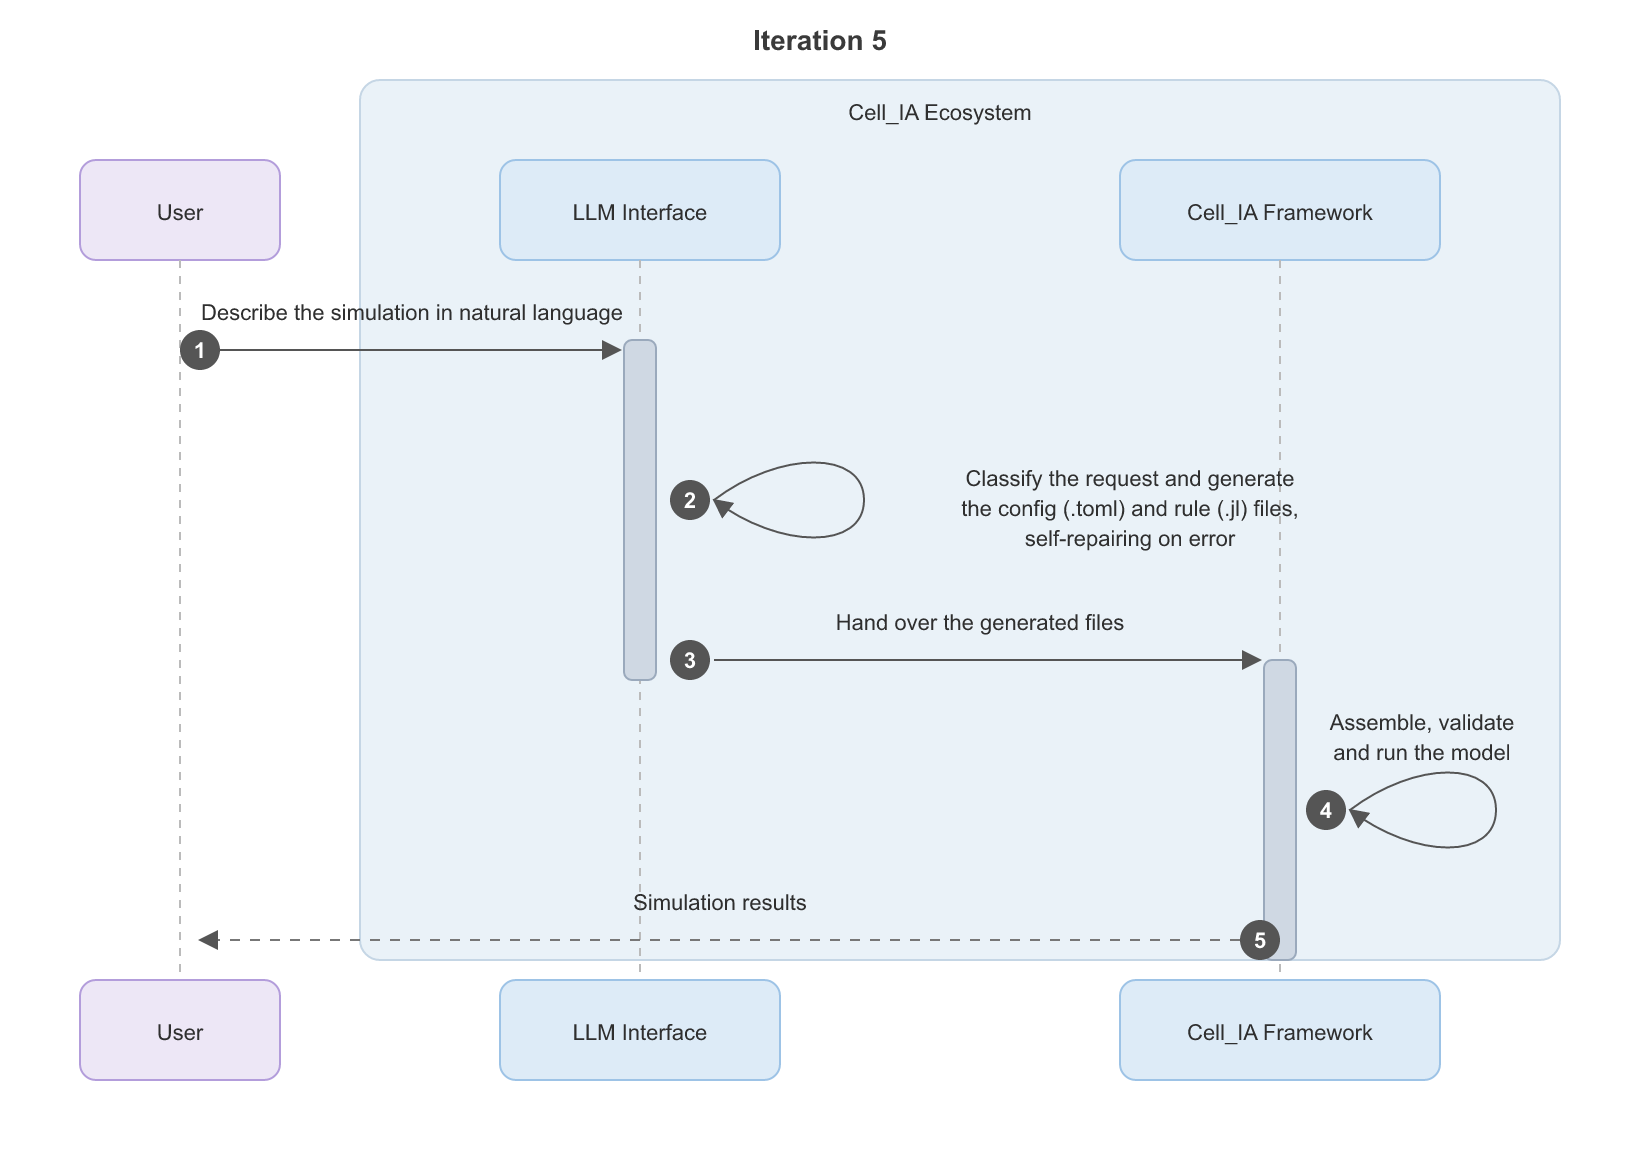
\includegraphics[width=1\textwidth]{iteration5.png}
\caption{Diagrama de secuencia, simplificado, de la generación de simulaciones mediante el LLM. El usuario describe la simulación en lenguaje natural; la interfaz con el modelo de lenguaje clasifica la petición (\emph{router}) y genera los archivos de configuración (\texttt{.toml}) y de reglas (\texttt{.jl}), reparándolos automáticamente ante errores de validación o de ejecución; por último, el framework Cell\_IA ensambla, valida y ejecuta el modelo y devuelve los resultados al usuario.}
\label{fig:seq_iter5}
\end{figure}

\subsubsection{Modelo de lenguaje utilizado: especificaciones técnicas}
\label{sec:llm_specs}
El módulo \texttt{LLMBuilder} utiliza el modelo \textit{Qwen2.5-Coder-1.5B} \cite{ref_qwen} en su variante cuantizada \textit{qwen2.5-1.5b-coder-q4\_k\_m.gguf}. La elección de este modelo responde a criterios de eficiencia local y orientación a generación de código:

\begin{itemize}
    \item \textbf{Arquitectura y tamaño:} Modelo de la familia Qwen2.5-Coder de Alibaba Cloud, con 1.5 mil millones de parámetros. Fue preentrenado específicamente sobre corpus de código fuente en múltiples lenguajes de programación, incluyendo Julia, lo que mejora la calidad de los archivos generados (\texttt{.toml} y \texttt{.jl}) frente a modelos de propósito general de tamaño equivalente.
    \item \textbf{Cuantización Q4\_K\_M:} El modelo se distribuye en formato GGUF con cuantización de 4 bits (esquema K-Quant medio, Q4\_K\_M), lo que permite ejecutarlo en CPU sin GPU dedicada, con un consumo de memoria de aproximadamente 1 GB. Esto hace viable su integración en la propia máquina del investigador sin dependencias de servicios en la nube.
    \item \textbf{Ejecución local:} Se ejecuta mediante \texttt{llama.cpp} o su equivalente en Julia, lo que garantiza la privacidad de los datos del usuario y la reproducibilidad de los resultados sin necesidad de conexión a APIs externas.
\end{itemize}

\subsubsection{Estrategia de \textit{prompt engineering} y orquestación}
\label{sec:prompt_eng}
La interacción con el LLM no se apoya en un único prompt monolítico ni en \textit{fine-tuning} del modelo, sino en una arquitectura de varios prompts especializados coordinados por una capa de orquestación que encadena clasificación, generación y reparación automática. El flujo, ilustrado en la Figura~\ref{fig:seq_iter5}, consta de dos llamadas al modelo. La primera es un \emph{prompt de enrutado} (Apéndice~\ref{prompt:router}), restringido por una gramática formal (Apéndice~\ref{prompt:gbnf}) que obliga al modelo a clasificar la petición, mediante un objeto JSON, en una de las cuatro categorías de simulación. Fijada la categoría, una segunda llamada emplea un megaprompt de generación formado por un núcleo común (Apéndice~\ref{prompt:core}) y el bloque específico de la categoría (Apéndices~\ref{prompt:grid} a \ref{prompt:hex}), que produce los archivos \texttt{config.toml} y \texttt{rules.jl}. La separación es deliberada, ya que un modelo pequeño, de 1.5\,B de parámetros, acierta mucho más si resuelve primero qué tipo de problema se le plantea antes de afrontar la generación.

Sobre esta base, una capa de \textit{harness engineering} dota al sistema de capacidad de autocorrección. Como el modelo opera como una función de texto a texto sin acceso al entorno, esta capa intercepta su respuesta, aísla los bloques de código, escribe los archivos en disco y los somete a una validación estática; si esta falla, reinvoca al LLM realimentándolo con el mensaje de error concreto, hasta tres veces. Superada la validación, la simulación se ejecuta en un subproceso y, si Julia devuelve un error, su salida se reenvía de nuevo al modelo, hasta dos veces más. De este modo el sistema vuelve a llamar al modelo tantas veces como sea necesario, sin intervención humana.

\textbf{Análisis de resultados y conclusión del desarrollo:} Esta fase cierra el ciclo evolutivo local del framework proporcionando una interfaz de nivel superior. Al automatizar la generación del código técnico, el foco del usuario, técnico o no técnico, se desplaza desde la fricción de la sintaxis hacia el puro diseño experimental. 

\subsection{Iteración 6: Diagnóstico y optimización del motor de cómputo}
\label{sec:iteracion6}
La incorporación de los autómatas continuos en la Iteración~4 elevó la madurez del framework, pero también su coste computacional. Un estudio de rendimiento posterior, detallado en la Sección~\ref{sec:rendimiento_lenia}, reveló que el motor continuo de Cell\_IA era casi un orden de magnitud más lento que una implementación equivalente en Julia puro. Esta última iteración aborda, por tanto, dos tareas encadenadas: diagnosticar con rigor dónde se consumía ese tiempo y optimizar el motor en consecuencia, sin alterar la arquitectura modular ni la interfaz del framework.

Para localizar los cuellos de botella se recurrió al perfilador estadístico de la biblioteca estándar de Julia, el módulo \texttt{Profile}. A diferencia de un cronómetro, que solo mide el tiempo total, un perfilador estadístico muestrea la pila de llamadas miles de veces por segundo y, agregando esas muestras, indica en qué funciones permanece más tiempo el programa. Se perfiló únicamente el bucle de simulación, sobre una rejilla de $256\times256$ celdas, comparando las dos versiones del motor.

La Tabla~\ref{tab:profiling_lenia} reparte el tiempo de cómputo de un paso de Lenia antes y después de optimizar. En el motor original, buena parte del tiempo se gastaba en costes evitables y ajenos al cálculo: la lectura de los parámetros desde un diccionario sin tipar, que provocaba inestabilidad de tipos y suponía cerca de una quinta parte del tiempo; la presión sobre el recolector de basura, al reasignar el campo y sus transformadas en cada paso; el uso de una transformada de Fourier compleja, que duplica el trabajo frente a la real; y la comprobación de límites en el indexado de matrices.

\begin{table}[H]
\centering
\caption{Reparto del tiempo de cómputo de un paso de Lenia entre las operaciones principales, antes y después de la optimización, medido con el perfilador estadístico (rejilla $256\times256$, un hilo de CPU; valores aproximados). Los porcentajes son relativos al tiempo total de cada versión; como ese tiempo por paso se reduce unas cuatro veces al optimizar, una operación puede aumentar su porcentaje aunque su coste absoluto disminuya, como le ocurre a la transformada.}
\label{tab:profiling_lenia}
{\small
\begin{tabular}{@{}lcc@{}}
\toprule
\textbf{Operación} & \textbf{Antes} & \textbf{Después} \\ \midrule
Lectura de parámetros y agentes (\texttt{getproperty}) & 22\,\% & 14\,\% \\
Recolección de basura y gestión de memoria & $>$10\,\% & $\approx$0\,\% \\
Transformada de Fourier & 9\,\% & 13\,\% \\
Indexado de matrices con comprobación de límites & 6\,\% & $\approx$0\,\% \\
Empaquetado de valores (\textit{boxing}) & 2\,\% & $\approx$0\,\% \\
Escritura del estado a los agentes (\texttt{setproperty!}) & 2\,\% & 15\,\% \\
Recorrido del contenedor de agentes & 4\,\% & 19\,\% \\ \bottomrule
\end{tabular}
}
\end{table}

Tras la optimización esos costes prácticamente desaparecen, y el tiempo restante se concentra en lo irreducible del modelado basado en agentes: leer y escribir el estado de cada agente y recorrer el contenedor de agentes pasan a suponer cerca de la mitad del tiempo. El perfilado confirma así que el sobrecoste de Cell\_IA nunca estuvo ni en Julia ni en la transformada, sino en el trasvase del estado entre los 65.536 agentes y la rejilla en cada paso.

Guiada por este diagnóstico, la reescritura del bucle interno atacó exactamente esas causas. La Sección~\ref{sec:optimizacion_cellia} describe las mejoras y cuantifica la aceleración resultante, de entre 2,9 y 3,8 veces según el tamaño de la rejilla, conservando la equivalencia numérica. Es destacable que fue posible acelerar el motor de forma sustancial sin tocar su estructura modular ni su interfaz, ya que la optimización quedó confinada al bucle interno de la regla de Lenia.

\subsection{Fase de despliegue y distribución del framework}
Una vez consolidada la arquitectura técnica y validadas las iteraciones de desarrollo a nivel local, la última etapa para convertir a Cell\_IA en una herramienta de impacto es su despliegue y apertura a la comunidad. En el ecosistema de Julia, la distribución de software obedece a unos estándares de empaquetado que garantizan que cualquier investigador del mundo pueda reproducir los mismos resultados en su propia máquina.\\

El despliegue de Cell\_IA como librería pública en GitHub se articuló en varias fases metodológicas. En primer lugar, se procedió a la estructuración del repositorio definiendo los archivos \texttt{Project.toml} y \texttt{Manifest.toml}. Estos ficheros contienen la identidad del paquete (versión, UUID único) y resuelven el árbol exacto de dependencias necesarias (como \texttt{Agents.jl}, \texttt{LinearAlgebra.jl}, \texttt{CairoMakie.jl} o \texttt{Statistics.jl}), evitando así problemas de compatibilidad futura.\\

A continuación, la interacción del desarrollador con los sistemas de Integración Continua (CI/CD) permite la automatización de la calidad del código. Se configurarán (TODAVIA NO LO HE HECHO) acciones de GitHub (GitHub Actions) que ejecutan una batería de pruebas unitarias contenidas en el módulo nativo de \texttt{Test} de Julia cada vez que se introduce una modificación al código. Asimismo, se desplegará una primera versión de la documentación hecha a mano, para que posteriormente pueda ser automatizada utilizando la herramienta \texttt{Documenter.jl}, permitiendo que los manuales de usuario y las referencias de la API de cada módulo se actualicen y publiquen.\\

Finalmente, la disponibilidad pública se concreta permitiendo que cualquier usuario abra la consola interactiva de Julia (REPL) y ejecute directamente el comando \texttt{using Pkg; Pkg.add("Cell\_IA")}).

\section{Caso de estudio: Resiliencia y estabilidad en sistemas continuos bajo perturbaciones estocásticas}

Para validar la versatilidad y robustez del framework desarrollado, se plantea un experimento de``estrés'' sobre un sistema continuo basado en el modelo Lenia. El objetivo es evaluar la capacidad de las estructuras biomorfas emergentes y ver si son capaces de conservar su organización y comportamiento frente a la introducción de ruido ambiental, es decir, cuando el entorno se vuelve inestable o impredecible.

\subsection{Metodología: Diseño asistido por LLM y flujo de trabajo}
El experimento se estructura en tres fases que integran el uso de Modelos de Lenguaje de Gran Escala (LLM) como catalizadores del diseño, seguidos de la ejecución técnica en el framework:

\begin{enumerate}
    \item \textbf{Fase de diseño (LLM):} Se utiliza un LLM como ``arquitecto biológico'' para generar el conjunto de parámetros $(\mu, \sigma)$ del kernel y la configuración de la función de crecimiento $G$. Esta aproximación permite testear si el framework es capaz de interpretar preguntas o descripciones conceptuales de alto nivel (ej. ``¿Puedo crear un sistema continuo donde aparezcan formas vivas y añadir pequeñas perturbaciones aleatorias en el espacio para ver si sobreviven o se desintegran?'') y traducirlas a dinámicas estables.
    \item \textbf{Fase de Simulación:} El framework debería de instanciar un espacio continuo $\mathcal{L} \in \mathbb{R}^2$ con condiciones de contorno periódicas y aplicar el motor de convolución basado en FFT para observar la emergencia de ``seres vivos''.
    \item \textbf{Fase de Perturbación:} Una vez establecida una estructura estable, se introduciría un campo de ruido blanco $\eta$ tal que el nuevo estado sea $A'_{t} = A_{t} + \eta$, donde $\eta \sim \mathcal{N}(0, \sigma_{\text{ruido}})$.
\end{enumerate}

\subsection{Planteamiento del experimento}
La pregunta de investigación que guía este caso de estudio es: ``¿Es posible la persistencia de formas de vida artificial en un entorno continuo cuando este es sometido a perturbaciones aleatorias en su espacio de estados?''.\\

Para responder a esto, se define un escenario donde se monitoriza la ``energía total'' del sistema (definida como el sumatorio de los estados de las celdas $E = \sum A_{i,j}$). Se establecen dos criterios de salida:
\begin{itemize}
    \item \textbf{Supervivencia (Robustez):} La estructura deforma su morfología para absorber el ruido pero recupera su entropía original o mantiene su cohesión estructural.
    \item \textbf{Desintegración (Colapso):} El ruido rompe el acoplamiento espacial, haciendo que la densidad del sistema se disipe hacia cero o vaya directa hacia la saturación ($\text{clip} \to 1$).
\end{itemize}



\subsection{Resultados esperados y verificación del framework}
Este experimento sirve como una prueba de validación integral (End-to-End) del software:
\begin{itemize}
    \item \textbf{Flexibilidad de Usuario:} Demuestra que un usuario externo, utilizando el LLM como interfaz, puede orquestar simulaciones de alta complejidad sin manipular directamente el motor de renderizado o de cálculo.
    \item \textbf{Capacidad Analítica:} El framework debe permitir la extracción de datos en tiempo real para observar el momento exacto en el que una ``forma de vida'' sucumbe a la entropía del sistema, cumpliendo así con los estándares de una herramienta de investigación científica.
\end{itemize}

\subsection{Resultados del caso de estudio sobre la resiliencia y estabilidad}

La ejecución del experimento se llevó a cabo de forma íntegra sobre el framework, materializando las tres fases descritas en la metodología y registrando la evolución temporal de la energía total $E_t = \sum_{i,j} A_{i,j}$ y del número de celdas activas (celdas con $A_{i,j} > \varepsilon$, con $\varepsilon = 10^{-3}$) como indicador de la cohesión estructural. Todos los resultados son reproducibles a partir de una única semilla del generador de números aleatorios, ya que tanto la inicialización como el campo de ruido se extraen del generador interno del modelo, esto garantiza, además, que la trayectoria empleada para el análisis cuantitativo y la generada para el vídeo sean idénticas.

\subsubsection{Realización técnica de las tres fases}

El espacio continuo $\mathcal{L}$ se realizó, siguiendo la práctica canónica del modelo Lenia, como una rejilla periódica de $128 \times 128$ celdas cuyo estado es un valor continuo $A_{i,j} \in [0,1]$ ($\mathtt{Float64}$). Es decir, lo continuo es el espacio de estados, no las posiciones: esta discretización es precisamente la que permite aplicar el motor de convolución basado en la Transformada Rápida de Fourier (FFT), pues $K \circledast A$
se calcula como $U = \mathrm{Re}\big(\mathcal{F}^{-1}(\mathcal{F}(A)\cdot \mathcal{F}(K))\big)$ sobre una malla regular. El kernel $K$ se precomputa una sola vez al inicializar el modelo, y la evolución sigue la regla
\[
    A_{t+\Delta t} = \mathrm{clip}\big(A_t + \Delta t \cdot G(K \circledast A_t),\; 0,\; 1\big),
    \qquad
    G(u) = 2\exp\!\left(-\frac{(u-\mu)^2}{2\sigma^2}\right) - 1 .
\]

\textbf{Fase de diseño (LLM).} La interpretación de la pregunta conceptual de alto nivel se delegó en el modelo de lenguaje local. A partir del enunciado en lenguaje natural, un agente router clasificó la petición en la categoría \texttt{continuous\_field} y un segundo paso de generación produjo el fichero de configuración \texttt{TOML} con los parámetros del kernel $(\mu, \sigma)$, la función de crecimiento $G$ y los
parámetros de la perturbación. El sistema incorpora un bucle de validación y reparación: en el primer intento, el LLM ubicó incorrectamente las métricas de nivel modelo
($\texttt{total\_energy}$, $\texttt{active\_cells}$) en el canal de datos por agente
($\texttt{adata}$) en lugar del canal de modelo ($\texttt{mdata}$), el validador estático
detectó la inconsistencia, devolvió un mensaje correctivo y el modelo regeneró una
configuración válida en el segundo intento, sin intervención humana. Este episodio es, en sí
mismo, una validación del flujo asistido por LLM: el sistema no solo genera, sino que se autocorrige.\\

\textbf{Fase de simulación.} Para disponer de una estructura estable bien definida que perturbar,
se sembró el patrón canónico \emph{orbium} centrado en la rejilla, bajo los parámetros propios de dicha criatura ($\mu = 0.15$, $\sigma = 0.015$, radio del kernel $R = 13$, $\Delta t = 0.1$,
kernel gaussiano). Partiendo de una energía inicial $E_0 \approx 75.1$, la estructura disipó un $\sim 5.5\%$ de su masa durante los primeros $\sim 25$ pasos, relajándose hacia su atractor exacto, y a continuación mantuvo una energía constante $E \approx 71$ (con $\approx 208$ celdas activas) de forma indefinida, confirmando la emergencia de un ``ser vivo'' estable y coherente. La Figura~\ref{fig:orbium_normal} muestra tres instantes de esta evolución en ausencia de perturbación.

\begin{figure}[H]
\centering
\begin{subfigure}[b]{0.32\textwidth}
    \centering
    
\includegraphics[width=\textwidth]{MIA-thesis-latex/orbium_energia_normal_inicial.png}
    \caption{Estado inicial ($t=0$).}
    \label{fig:orbn_ini}
\end{subfigure}
\hfill
\begin{subfigure}[b]{0.32\textwidth}
    \centering
    
\includegraphics[width=\textwidth]{MIA-thesis-latex/orbium_energia_normal_medio.png}
    \caption{Estado intermedio.}
    \label{fig:orbn_med}
\end{subfigure}
\hfill
\begin{subfigure}[b]{0.32\textwidth}
    \centering
    
\includegraphics[width=\textwidth]{MIA-thesis-latex/orbium_energia_normal_final.png}
    \caption{Estado final (estable).}
    \label{fig:orbn_fin}
\end{subfigure}
\caption{Evolución del orbium en ausencia de perturbación: partiendo de su estado inicial, la estructura se relaja hacia su atractor y conserva su forma de manera indefinida.}
\label{fig:orbium_normal}
\end{figure}

\subsubsection{Fase de perturbación: transición de la robustez al colapso}

Una vez estabilizada la estructura, se inyectó el campo de ruido blanco $A'_t = \mathrm{clip}(A_t + \eta,\,0,\,1)$, con $\eta \sim \mathcal{N}(0, \sigma_{\text{ruido}})$,
de forma sostenida a partir de un paso $K$. La perturbación se restringió al soporte del
organismo (celdas con $A_{i,j} > \varepsilon$) por una razón física relevante: el operador de
recorte $\mathrm{clip}(\cdot, 0, 1)$ no conserva la energía y es asimétrico cerca de los
límites (una celda en $0$ solo puede aumentar), por lo que aplicar ruido sobre el fondo vacío sesgaría sistemáticamente $E$ al alza y podría nuclear estructura falsa, contaminando la
medición.\\

Para localizar el régimen de transición se realizó un barrido de la amplitud del ruido. La
Tabla~\ref{tab:barrido_sigma} resume el estado del sistema tras la perturbación: para amplitudes
bajas la estructura absorbe el ruido y conserva su energía y su cohesión (supervivencia),
mientras que por encima de un umbral crítico el ruido rompe el acoplamiento espacial inducido por
la convolución y la densidad se disipa hacia cero (desintegración).

\begin{table}[h]
\centering
\begin{tabular}{cccl}
\hline
$\sigma_{\text{ruido}}$ & Energía final $E$ & Celdas activas & Desenlace \\
\hline
0.02 & $\approx 70.7$ & $199$ & Supervivencia (robustez) \\
0.04 & $\approx 71.6$ & $200$ & Supervivencia (robustez) \\
0.08 & $0.0$          & $0$   & Desintegración (colapso) \\
0.15 & $0.0$          & $0$   & Desintegración (colapso) \\
\hline
\end{tabular}
\caption{Estado del orbium tras someterse a ruido sostenido, en función de la amplitud
$\sigma_{\text{ruido}}$. El umbral crítico de robustez se sitúa entre $0.04$ y $0.08$.}
\label{tab:barrido_sigma}
\end{table}

\begin{figure}[H]
\centering
\begin{subfigure}[b]{0.32\textwidth}
    \centering
    
\includegraphics[width=\textwidth]{MIA-thesis-latex/orbium_energia_perturbacion_inicial.png}
    \caption{Estado inicial ($t=0$).}
    \label{fig:orbp_ini}
\end{subfigure}
\hfill
\begin{subfigure}[b]{0.32\textwidth}
    \centering
    
\includegraphics[width=\textwidth]{MIA-thesis-latex/orbium_energia_perturbacion_medio.png}
    \caption{Inicio de la perturbación ($t=K$).}
    \label{fig:orbp_med}
\end{subfigure}
\hfill
\begin{subfigure}[b]{0.32\textwidth}
    \centering
    
\includegraphics[width=\textwidth]{MIA-thesis-latex/orbium_energia_perturbacion_final.png}
    \caption{Estado final.}
    \label{fig:orbp_fin}
\end{subfigure}
\caption{Evolución del orbium sometido a una perturbación estocástica sostenida ($\sigma_{\text{ruido}}=0{,}04$): el organismo absorbe el ruido inyectado y mantiene su cohesión, un desenlace de supervivencia.}
\label{fig:orbium_perturbado}
\end{figure}

Este resultado responde afirmativamente, y con matices cuantitativos, a la pregunta de
investigación: la persistencia de formas de vida artificial bajo perturbaciones estocásticas es posible, pero está acotada por una amplitud crítica de ruido. La existencia de este umbral admite una interpretación dinámica clara: el flujo de Lenia se comporta como una contracción hacia su atractor, capaz de dispar las perturbaciones de alta frecuencia mientras su tasa de inyección sea inferior a la tasa de relajación del sistema. Superado el umbral, las perturbaciones degradan la coherencia espacial más rápido de lo que el crecimiento puede restaurarla, desencadenando un colapso irreversible.\\

En el escenario nominal del experimento ($\sigma_{\text{ruido}} = 0.04$, perturbación sostenida
desde $K = 120$ durante $400$ pasos), el clasificador automático emitió el veredicto de
supervivencia: la energía media de la línea base previa a la perturbación
($E_{\text{base}} = 71.13$) se conservó tras la inyección de ruido ($E_{\text{final}} = 71.27$),
como se aprecia en la Figura~\ref{fig:orbium_energia}. La Figura~\ref{fig:orbium_perturbado} muestra el organismo antes de la perturbación, en el instante en que se inyecta y al final del experimento.

\begin{figure}[h]
\centering

\includegraphics[width=0.85\textwidth]{lenia_energy.png}
\caption{Evolución de la energía total $E_t$ (arriba) y de las celdas activas (abajo) para el
orbium con $\sigma_{\text{ruido}} = 0.04$. La línea vertical discontinua marca el inicio de la
perturbación ($K = 120$) y la línea de puntos la energía de la línea base. La estructura absorbe
el ruido manteniéndose en torno a su línea base: supervivencia.}
\label{fig:orbium_energia}
\end{figure}

\subsubsection{Validación end-to-end a través del LLM}

Como prueba de la flexibilidad de usuario, se ejecutó adicionalmente la simulación generada íntegramente por el LLM a partir de la pregunta en lenguaje natural, sin que el usuario
manipulase el motor de cálculo ni de renderizado. La configuración generada empleó una inicialización aleatoria uniforme del campo (en lugar del sembrado de un organismo concreto, que
constituye conocimiento específico del experimento no inferible por el modelo). El análisis de su evolución reveló una dinámica físicamente coherente y de notable riqueza
(Figura~\ref{fig:llm_energia}):

\begin{enumerate}
    \item \textbf{Colapso transitorio:} partiendo de $E_0 \approx 8223$ (campo aleatorio, con la
    práctica totalidad de las celdas activas), la energía se desplomó hasta un mínimo
    $E \approx 1500$ en torno al paso $15$. Ello se debe a que la densidad media inicial
    ($\approx 0.5$) queda muy por encima de la estrecha ventana de crecimiento centrada en
    $\mu = 0.15$, de modo que $G(u) \approx -1$ en casi todo el dominio y la masa decae.
    \item \textbf{Autoorganización:} a medida que la densidad descendió, ciertas regiones
    alcanzaron la ventana de crecimiento y el sistema se reorganizó espontáneamente en una
    estructura emergente persistente (una ``sopa'' de patrones), estabilizándose en una meseta de
    $E \approx 3500$ y $\approx 4000$ celdas activas hacia el paso $100$.
    \item \textbf{Respuesta a la perturbación:} la inyección de ruido en $K = 120$ produjo
    únicamente una leve fluctuación de la que el sistema se recuperó ($E_{\text{base}} = 3237 \to
    E_{\text{final}} = 3562$), emitiéndose nuevamente un veredicto de supervivencia.
\end{enumerate}

\begin{figure}[h]
\centering

\includegraphics[width=0.85\textwidth]{lenia_noisy_energy.png}
\caption{Evolución de la simulación diseñada por el LLM (inicialización aleatoria). Se observa
el colapso transitorio, la posterior autoorganización hacia una meseta estable y la supervivencia
de la estructura emergente frente a la perturbación inyectada en $K = 120$.}
\label{fig:llm_energia}
\end{figure}

Es relevante destacar que ambas configuraciones, el orbium sembrado y la sopa emergente del
LLM, constituyen estudios de resiliencia válidos: la primera ofrece una demostración nítida sobre
un organismo individual bien definido, mientras que la segunda, más abierta, encaja de forma
natural con la formulación original de la pregunta de investigación sobre la persistencia de
``formas de vida'' emergentes.

\subsubsection{Verificación del framework y consideraciones}

Los resultados confirman los dos objetivos de validación planteados. En cuanto a la
flexibilidad de usuario, se demostró que una pregunta conceptual en lenguaje natural se traduce, a través del LLM como interfaz, en una simulación compleja y ejecutable, incluyendo la autocorrección de errores de configuración mediante el bucle de validación. En cuanto a la capacidad analítica, el framework permitió extraer la serie temporal de la energía y la
cohesión en cada paso y clasificar automáticamente el desenlace, identificando el régimen exacto (supervivencia frente a colapso) y la amplitud de ruido que separa ambos comportamientos.\\

Desde el punto de vista del diseño del software, la integración del experimento respetó la modularidad del framework: las piezas genéricas y reutilizables (la extracción de métricas escalares calculadas, el paso de evolución con forzamiento estocástico opcional, inerte cuando $\sigma_{\text{ruido}} = 0$,  y las métricas de retícula) se incorporaron al motor, mientras que
todo lo específico del experimento (el patrón \emph{orbium}, la configuración concreta y el análisis del veredicto) permaneció en ficheros de usuario, sin contaminar el núcleo de cálculo.\\

Conviene, por último, señalar las limitaciones del estudio. El espacio ``continuo'' es en rigor
una retícula discreta de alta resolución que porta un estado continuo, condición necesaria para
el motor FFT. El umbral crítico de ruido se ha acotado de forma gruesa (entre $0.04$ y $0.08$) y
admitiría un barrido más fino para su determinación precisa. Finalmente, la fase de diseño asistido
por LLM se validó en su modalidad de parametrización (selección de $\mu$, $\sigma$ y de los
parámetros de perturbación), la autoría completa de una función de crecimiento $G$ novedosa por
parte del modelo, aunque soportada por la arquitectura del generador, queda como línea de trabajo
futura.


\section{Estudio de rendimiento comparativo de Lenia en C, Python, Julia y Cell\_IA}
\label{sec:rendimiento_lenia}
Uno de los motivadores clave para desarrollar Cell\_IA en Julia es su potencial de rendimiento. Para cuantificar esta ventaja se plantea un experimento de rendimiento puro que compara la ejecución de Lenia \cite{ref_lenia} en distintos lenguajes y entornos. En todos los casos se excluye el tiempo de renderizado y visualización para medir únicamente el coste computacional del motor de simulación: la convolución circular por FFT, la función de crecimiento y el recorte de estados al intervalo $[0,1]$.\\

\subsection{Planteamiento y diseño del experimento}
\label{sec:rendimiento_planteamiento}

La elección de las implementaciones a comparar parte de revisar las que ya existen. El repositorio oficial de Lenia\footnote{\url{https://github.com/Chakazul/Lenia}} reúne versiones en varios lenguajes, y de todas ellas la más extendida en la comunidad investigadora es la de Python con NumPy/SciPy, que se toma aquí como referencia del flujo de trabajo habitual. También se consideraron proyectos de aceleración por GPU como cuLenia\footnote{\url{https://github.com/StefanBornhofen/cuLenia}}, escrito en CUDA C++.\\

A partir de ahí se seleccionaron seis implementaciones que cubren el espectro de interés. Como referencia de bajo nivel se emplea una versión en C apoyada en FFTW. Para conocer el techo del propio lenguaje Julia, al margen del framework, se incluye una versión en Julia puro con FFTW.jl, y junto a ella se mide Cell\_IA, es decir, el motor del framework tal cual, construido sobre Agents.jl y FFTW.jl. Del lado de Python se consideran dos variantes: la habitual con NumPy, que internamente recurre a pocketfft, y otra con pyFFTW, que conserva Python pero sustituye el backend de transformada por FFTW. Por último, una versión en Python con CuPy ejecuta el mismo algoritmo sobre la GPU mediante cuFFT.\\

Cada una de estas parejas responde a una pregunta concreta. Comparar Julia puro con Cell\_IA permite separar lo que cuesta el lenguaje de lo que cuesta la abstracción de agentes del framework. Comparar NumPy con pyFFTW aísla el sobrecoste del intérprete de Python del que introduce el backend de FFT, puesto que ambas comparten todo salvo la biblioteca de transformada. Además, C y Julia se enlazan deliberadamente contra el mismo binario de FFTW, el que distribuye FFTW\_jll, de modo que su diferencia refleje únicamente el coste del lenguaje y no el de la transformada, que es idéntica en ambos. En lo que respecta a la GPU, cuLenia se descartó como competidor directo porque exige hardware NVIDIA específico y no ofrece alternativa en CPU, en su lugar se recurre a CuPy, que ejecuta exactamente el mismo algoritmo sobre la tarjeta gráfica.\\

Para que la comparación sea justa y reproducible, todas las implementaciones ejecutan el mismo algoritmo (kernel gaussiano canónico con $\mu=0.15$, $\sigma=0.017$, $dt=0.1$, radio $R=13$), en doble precisión, partiendo de la misma semilla determinista, sin generación de números aleatorios y con un único hilo de CPU. La carga de trabajo es el orbium, el organismo planeador canónico de Lenia, teselado a densidad constante (un orbium por cada celda de $64\times64$: 4 en $128^2$, 16 en $256^2$ y 64 en $512^2$), lo que mantiene el espacio poblado de forma realista a cualquier escala sin alterar la dinámica. Antes de cada medición se realiza un calentamiento que descarta la compilación JIT de Julia, la creación de los planes FFTW y los fallos de página iniciales, el cronómetro envuelve exclusivamente el bucle de pasos, y en la GPU se sincroniza el dispositivo antes y después del bucle por ser las operaciones CUDA asíncronas. La correctitud se verificó comprobando que las seis implementaciones producen la misma energía total $E=\sum A_{ij}$ a horizonte corto, las pequeñas divergencias a 1000 pasos (inferiores a $10^{-9}$) se deben a la no-asociatividad de la aritmética en coma flotante entre transformadas distintas y no afectan a la medida de tiempos.\\

Antes de continuar, es necesario hacer una observación metodológica: el procesador es de bajo consumo (15W) y bajo carga sostenida presenta estrangulamiento térmico, una especie de mecanismo de defensa que presentan los componentes electrónicos para evitar daños permanentes reduciendo el rendimiento, por lo que las cifras absolutas a $512^2$ son algo mayores que en ráfagas cortas, y, como todas las implementaciones se ejecutaron en la misma máquina, mismas condiciones y de forma secuencial, la comparación relativa se mantiene válida.

\subsection{Resultados}
\label{sec:rendimiento_resultados}

La Tabla~\ref{tab:rendimiento_lenia} resume los resultados y la Figura~\ref{fig:orbium_grids} ilustra la carga de trabajo, con orbiums teselados, empleada en cada tamaño de rejilla.

\begin{table}[H]
\centering
\caption{Rendimiento del motor de Lenia sin visualización (doble precisión, 1 hilo de CPU salvo la fila GPU). Mediana de 5 ejecuciones de 1000 pasos, en ms/paso, el tiempo total para 1000 pasos en segundos coincide numéricamente con la cifra de ms/paso. Máquina: Intel Core i7-8565U, GPU NVIDIA GeForce MX130.}
\label{tab:rendimiento_lenia}
\begin{tabular}{@{}llccc@{}}
\toprule
\textbf{Implementación} & \textbf{Disp.} & \textbf{128$\times$128} & \textbf{256$\times$256} & \textbf{512$\times$512} \\ \midrule
C (FFTW, referencia)            & CPU & 0.626 & 3.234 & 14.309 \\
Julia puro (FFTW.jl)            & CPU & 0.702 & 3.411 & 14.481 \\
Cell\_IA (Agents.jl + FFTW.jl)  & CPU & 5.842 & 30.633 & 147.659 \\
Python (NumPy / pocketfft)      & CPU & 1.753 & 8.204 & 39.270 \\
Python (pyFFTW / FFTW)          & CPU & 0.885 & 5.663 & 25.933 \\
Python (CuPy / cuFFT)           & GPU & 0.868 & 1.687 & 7.097 \\ \bottomrule
\end{tabular}
\end{table}

\begin{figure}[H]
\centering
\begin{subfigure}[b]{0.32\textwidth}
    \centering
    \includegraphics[width=\textwidth]{grid128x128.png}
    \caption{$128\times128$ (4 orbiums).}
    \label{fig:orbium128}
\end{subfigure}
\hfill
\begin{subfigure}[b]{0.32\textwidth}
    \centering
    \includegraphics[width=\textwidth]{grid256x256.png}
    \caption{$256\times256$ (16 orbiums).}
    \label{fig:orbium256}
\end{subfigure}
\hfill
\begin{subfigure}[b]{0.32\textwidth}
    \centering
    \includegraphics[width=\textwidth]{grid512x512.png}
    \caption{$512\times512$ (64 orbiums).}
    \label{fig:orbium512}
\end{subfigure}
\caption{Campo de Lenia con orbiums teselados a densidad constante (un orbium
por celda de $64\times64$) para cada tamaño de rejilla evaluado en el
experimento de rendimiento. El teselado mantiene el campo poblado de forma
realista a toda escala sin alterar la dinámica.}
\label{fig:orbium_grids}
\end{figure}

Los datos confirman la hipótesis de partida. Julia, gracias a FFTW.jl y a la compilación JIT, alcanza el rendimiento de C tras el calentamiento, situándose entre un 1\,\% y un 12\,\% por encima, esa diferencia se reduce al crecer la rejilla, porque el coste pasa a estar dominado por la propia transformada, que es el mismo binario en ambos casos. Python queda por detrás debido al sobrecoste del intérprete: la comparación entre pyFFTW y NumPy revela que una parte de la diferencia se explica por el backend de FFT, mientras que la brecha restante de pyFFTW frente a C y Julia (en torno a $1{,}8\times$ a $512^2$) corresponde al coste del intérprete en las operaciones elemento a elemento. La GPU, pese a tratarse de una tarjeta modesta y con doble precisión limitada, resulta la más rápida en las rejillas mayores, en torno al doble que C a $256^2$ y $512^2$, porque ahí domina el paralelismo de la transformada. En $128^2$, en cambio, no compensa: el coste fijo de lanzar los núcleos de cómputo y de sincronizar el dispositivo pesa más que el trabajo útil. Dado que ese coste fijo es prácticamente independiente del tamaño del problema, cabe esperar que en rejillas todavía mayores su peso relativo siga disminuyendo frente a un volumen de cálculo creciente, de modo que la ventaja de la GPU debería ampliarse. Por último, se verificó mediante monitorización de \texttt{nvidia-smi} que ninguna de las implementaciones de CPU, Cell\_IA incluida, utiliza la GPU, dado que FFTW.jl opera exclusivamente sobre el procesador.\\


Llama la atención el caso de Cell\_IA, entre ocho y diez veces más lento que Julia puro a pesar de compartir lenguaje y biblioteca de transformada. El análisis revela que ese sobrecoste no proviene de Julia ni de la FFT, sino de la abstracción de agentes: en cada paso el motor vuelca el estado de hasta 262\,144 agentes a una matriz y lo reescribe después, además de no reutilizar los planes de la transformada ni los buffers, y de incurrir en despacho dinámico al leer los parámetros de un diccionario sin tipado; el perfilado de la Iteración~6 (Sección~\ref{sec:iteracion6}) lo corrobora función a función. Conviene además mencionar de nuevo que el procesador es de bajo consumo (15\,W) y bajo carga sostenida presenta limitación térmica.

\subsection{Optimización del motor de Cell\_IA}
\label{sec:optimizacion_cellia}
A la vista de estos resultados se optimizó el motor de Lenia de Cell\_IA, con la restricción de no alterar su arquitectura: la simulación se sigue describiendo en TOML, el estado continúa residiendo en los agentes y la función de regla conserva su nombre y su semántica, de modo que cualquier configuración existente funciona igual que antes. Las mejoras son internas al bucle caliente: se emplea la transformada de Fourier real en lugar de la compleja, que reduce a la mitad el trabajo y la memoria, se precomputan y reutilizan los planes FFTW y los buffers en lugar de reasignarlos en cada paso, y se introduce una barrera de tipos que elimina el despacho dinámico debido al diccionario de propiedades. La Tabla~\ref{tab:optimizacion_cellia} recoge el efecto de estas mejoras, cuya equivalencia numérica con la versión original se verificó comprobando que la energía final coincide.

\begin{table}[H]
\centering
\caption{Efecto de la optimización del motor de Lenia en Cell\_IA, manteniendo intacta su estructura modular y su interfaz. Mediana de ms/paso (1000 pasos, 1 hilo de CPU, doble precisión).}
\label{tab:optimizacion_cellia}
\begin{tabular}{@{}lccc@{}}
\toprule
\textbf{Versión de Cell\_IA} & \textbf{128$\times$128} & \textbf{256$\times$256} & \textbf{512$\times$512} \\ \midrule
Original (FFT compleja, sin planes ni buffers)        & 5.842 & 30.633 & 147.659 \\
Optimizada (FFT real, planes y buffers, tipos fijos)  & 1.854 & 7.968  & 51.168  \\ \midrule
Aceleración                                           & 3.15$\times$ & 3.84$\times$ & 2.89$\times$ \\ \bottomrule
\end{tabular}
\end{table}

Con estas modificaciones Cell\_IA pasa de ser entre ocho y diez veces más lento que Julia puro a serlo solo entre dos y tres veces y media, igualando o incluso superando a la implementación habitual en Python con NumPy pese a arrastrar toda la maquinaria del modelado basado en agentes. El sobrecoste que permanece corresponde al trasvase del estado entre los agentes y la rejilla en cada paso, un coste inherente al paradigma de modelado basado en agentes y no al lenguaje, que solo podría eliminarse renunciando a almacenar el estado en los agentes y, con ello, a la generalidad y virtud del framework.




\section{Evaluation or discussion of results}
\label{sec:evaluacion}

\section{Conclusions}
\label{sec:conclusiones}
Este Trabajo de Fin de Máster ha presentado Cell\_IA, un framework modular en Julia para la simulación de autómatas celulares y modelos basados en agentes. A lo largo del desarrollo se ha construido, de forma incremental, una arquitectura de módulos desacoplados que permite definir simulaciones de manera declarativa, sin modificar el núcleo del sistema, y que cubre desde los autómatas discretos clásicos, como el Juego de la Vida, hasta generalizaciones continuas de alto coste computacional, como Lenia.

Las aportaciones principales se pueden resumir en cuatro puntos. En primer lugar, una arquitectura modular y parametrizable mediante archivos TOML que soporta distintos tipos de estado y topologías espaciales, incluida una rejilla hexagonal con métricas correctas que cubre una carencia del ecosistema de Agents.jl. En segundo lugar, una implementación nativa de Lenia en Julia basada en convolución por FFT que, tras la optimización descrita en la Iteración~6, alcanza un rendimiento solo entre dos y tres veces y media inferior al de Julia puro, pese a conservar toda la generalidad del paradigma de agentes. En tercer lugar, una interfaz de generación de simulaciones mediante un LLM local, que traduce descripciones en lenguaje natural a configuraciones ejecutables a través de una arquitectura de varios prompts con autocorrección. Por último, la validación del conjunto mediante un caso de estudio sobre la resiliencia de estructuras de Lenia frente a perturbaciones estocásticas, que demostró la capacidad analítica y la flexibilidad de la herramienta de extremo a extremo.

En conjunto, el framework cumple el objetivo de equilibrar eficiencia computacional, flexibilidad y accesibilidad, ofreciendo un único entorno en el que un investigador puede transitar entre modelos discretos y continuos y en el que un usuario sin perfil técnico puede lanzar simulaciones complejas sin escribir código.

\subsection{Trabajo futuro}
El desarrollo deja abiertas numerosas líneas de trabajo, tanto de ampliación del propio framework como de aplicación a problemas reales.

En cuanto a las capacidades del framework, se plantean las siguientes líneas:
\begin{itemize}
    \item Mejorar el generador de simulaciones asistido por LLM, empleando modelos más capaces o ajustados al dominio, y ampliar su alcance para que diseñe funciones de crecimiento y reglas novedosas, y no solo parametrizaciones de las ya existentes.
    \item Incorporar espacios tridimensionales (3D) que permitan simular fenómenos volumétricos, como el crecimiento de tejidos, la difusión en sólidos o estructuras biológicas espaciales.
    \item Explorar con mayor profundidad el espacio continuo, ampliando la familia de autómatas tipo Lenia con kernels y funciones de crecimiento multimodales y con varias especies que interactúan entre sí.
    \item Integrar algoritmos genéticos y evolutivos para descubrir de forma automática parámetros o criaturas estables, así como algoritmos de búsqueda de caminos (\textit{path finding}) para agentes con objetivos.
    \item Permitir inicializar la población pintando directamente sobre la rejilla, mediante un editor visual del estado inicial en los modelos discretos.
    \item Añadir interacción en tiempo real, de modo que el usuario pueda introducir perturbaciones u obstáculos durante la ejecución de simulaciones como Lenia y observar su respuesta de forma inmediata.
    \item Aprovechar la rejilla hexagonal, por su isotropía, para modelar moléculas y procesos biológicos sobre retículas más fieles a la geometría real.
    \item Acelerar el motor en GPU para las simulaciones continuas de gran tamaño, donde el paralelismo de la transformada resulta especialmente ventajoso.
    \item Completar el despliegue como paquete registrado de Julia, con integración continua, documentación automática y una batería de pruebas unitarias.
\end{itemize}

En cuanto a sus aplicaciones, la combinación de modelos discretos y continuos junto con la interfaz en lenguaje natural abre el uso del framework a múltiples disciplinas:
\begin{itemize}
    \item En biología y medicina, para modelar el crecimiento de tumores, la propagación de epidemias, la dinámica de poblaciones celulares o la morfogénesis y la embriogénesis artificial.
    \item En física y química, para simular procesos de difusión, sistemas de reacción-difusión, dinámica de fluidos en retícula o la formación de patrones.
    \item En ciencias sociales y economía, para estudiar fenómenos emergentes como la segregación urbana, la difusión de opiniones o el comportamiento de mercados.
    \item En vida artificial e inteligencia artificial, como entorno para descubrir criaturas y comportamientos emergentes y como banco de pruebas para agentes dotados de aprendizaje.
    \item En docencia y divulgación, gracias a la interfaz en lenguaje natural, que permite a estudiantes sin formación en programación experimentar con sistemas complejos.
\end{itemize}

\begin{thebibliography}{8}
\bibitem{ref_ca}
Bhattacharjee, K., Naskar, N., Roy, S., \& Das, S. (2020). A survey of cellular automata: types, dynamics, non-uniformity and applications. Natural Computing, 19(2), 433-461.
\doi{10.1007/s11047-018-9696-8}

\bibitem{ref_lenia}
Chan, B. W. C. (2018). Lenia-biology of artificial life. arXiv preprint arXiv:1812.05433. \doi{10.48550/arXiv.1812.05433}

\bibitem{ref_epi}
White, S. H., Del Rey, A. M., \& Sánchez, G. R. (2007). Modeling epidemics using cellular automata. Applied mathematics and computation, 186(1), 193-202. \doi{10.1016/j.amc.2006.06.126}

\bibitem{ref_grow}
Mordvintsev, A., Randazzo, E., Niklasson, E., \& Levin, M. (2020). Growing neural cellular automata. Distill, 5(2), e23. \doi{10.23915/distill.00023}

\bibitem{ref_gol}
Conway, J. (1970). Conway’s game of life. \doi{}

\bibitem{ref_abm}
Bonabeau, E. (2002). Agent-based modeling: Methods and techniques for simulating human systems. Proceedings of the national academy of sciences, 99(suppl\_3), 7280-7287. \doi{10.1073/pnas.082080899}

\bibitem{ref_societies}
Epstein, J. M., \& Axtell, R. (1996). Growing artificial societies: social science from the bottom up. Brookings Institution Press.

\bibitem{ref_marl}
Zhang, K., Yang, Z., \& Başar, T. (2021). Multi-agent reinforcement learning: A selective overview of theories and algorithms. Handbook of reinforcement learning and control, 321-384. \doi{10.1007/978-3-030-60990-0_12}

\bibitem{ref_llm}
Vaswani, A., Shazeer, N., Parmar, N., Uszkoreit, J., Jones, L., Gomez, A. N., ... \& Polosukhin, I. (2017). Attention is all you need. Advances in neural information processing systems, 30.

\bibitem{ref_llm2}
Brown, T., Mann, B., Ryder, N., Subbiah, M., Kaplan, J. D., Dhariwal, P., ... \& Amodei, D. (2020). Language models are few-shot learners. Advances in neural information processing systems, 33, 1877-1901.

\bibitem{ref_julia}
Bezanson, J., Edelman, A., Karpinski, S., \& Shah, V. B. (2017). Julia: A fresh approach to numerical computing. SIAM review, 59(1), 65-98. \doi{10.1137/141000671}

\bibitem{ref_netlogo}
Sklar, E. (2007). NetLogo, a multi-agent simulation environment. Artificial life, 13(3), 303-311. \doi{10.1162/artl.2007.13.3.303}

\bibitem{ref_mesa}
Ter Hoeven, E., Kwakkel, J., Hess, V., Pike, T., Wang, B., \& Kazil, J. (2025). Mesa 3: Agent-based modeling with Python in 2025. Journal of Open Source Software, 10(107), 7668. \doi{10.21105/joss.07668}

\bibitem{ref_mason}
Luke, S., Cioffi-Revilla, C., Panait, L., Sullivan, K., \& Balan, G. (2005). Mason: A multiagent simulation environment. Simulation, 81(7), 517-527. \doi{10.1177/0037549705058073}

\bibitem{ref_pettingzoo}
Terry, J., Black, B., Grammel, N., Jayakumar, M., Hari, A., Sullivan, R., ... \& Ravi, P. (2021). Pettingzoo: Gym for multi-agent reinforcement learning. Advances in Neural Information Processing Systems, 34, 15032-15043.
\doi{10.48550/arXiv.2009.14471}

\bibitem{ref_rlib}
Liang, E., Liaw, R., Nishihara, R., Moritz, P., Fox, R., Goldberg, K., ... \& Stoica, I. (2018, July). RLlib: Abstractions for distributed reinforcement learning. In International conference on machine learning (pp. 3053-3062). PMLR. \doi{10.48550/arXiv.1712.0938}

\bibitem{ref_asyn}
Schönfisch, B., \& De Roos, A. (1999). Synchronous and asynchronous updating in cellular automata. BioSystems, 51(3), 123-143. \doi{10.1016/S0303-2647(99)00025-8}

\bibitem{ref_llama}
Touvron, H., Lavril, T., Izacard, G., Martinet, X., Lachaux, M. A., Lacroix, T., ... \& Lample, G. (2023). Llama: Open and efficient foundation language models. arXiv preprint arXiv:2302.13971. \doi{10.48550/arXiv.2302.13971}

\bibitem{ref_qwen}
Hui, B., Yang, J., Cui, Z., Yang, J., Liu, L., Zhang, L., ... \& Lin, J. (2024). Qwen2.5-Coder Technical Report. arXiv preprint arXiv:2409.12186. \doi{10.48550/arXiv.2409.12186}

\bibitem{ref_blackbox}
Rudin, C. (2019). Stop explaining black box machine learning models for high stakes decisions and use interpretable models instead. Nature machine intelligence, 1(5), 206-215. \doi{10.48550/arXiv.1811.10154}

\bibitem{ref_scrum}
Schwaber, K., \& Sutherland, J. (2020). The scrum guide. Scrum Alliance, 21(19), 1.

\bibitem{ref_kanban}
Anderson, D. J. (2010). 
Kanban: Successful Evolutionary Change for Your Technology.

\bibitem{ref_agentsjl}
Datseris, G., Vahdati, A. R., \& DuBois, T. C. (2024). Agents. jl: a performant and feature-full agent-based modeling software of minimal code complexity. Simulation, 100(10), 1019-1031. \doi{10.1177/00375497211068820}

\bibitem{ref_schelling}
Schelling, T. C. (1971). Dynamic models of segregation. Journal of mathematical sociology, 1(2), 143-186. \doi{10.1080/0022250X.1971.9989794}

\bibitem{ref_economy}
Calero, M. P. (2022). Cellular Automata in the Economy: Application to the Behavior Theory of the Consumers. Economics, 11(1), 43-48. \doi{10.11648/j.eco.20221101.16}

\bibitem{ref_alife}
Langton, C. G. (2019). Artificial life. In Artificial life (pp. 1-47). Routledge.

\bibitem{ref_leniarepo}
Chan, B. W.-C. (2018). Lenia [Computer software]. \href{https://github.com/Chakazul/Lenia}{GitHub}.

\bibitem{ref_tumor}
Joachimczak, M., \& Wróbel, B. (2009, September). Evolution of the morphology and patterning of artificial embryos: scaling the tricolour problem to the third dimension. In European Conference on Artificial Life (pp. 35-43). Berlin, Heidelberg: Springer Berlin Heidelberg. \doi{10.1007/978-3-642-21283-3_5}

\bibitem{ref_greans}
Joachimczak, M., \& Wróbel, B. (2012). Evolution of robustness to damage in artificial 3-dimensional development. Biosystems, 109(3), 498-505. \doi{https://doi.org/10.1016/j.biosystems.2012.05.014}

\bibitem{ref_sistema_celular}
Fernández Blanco, E. (2010). Modelado de un sistema celular artificial para generación de formas y procesado de información. Universidade da Coruña.
\url{http://hdl.handle.net/2183/12353}

\bibitem{ref_wolfram}
Wolfram, S. (1983). Statistical mechanics of cellular automata. Reviews of Modern Physics, 55(3), 601–644.
\doi{10.1103/RevModPhys.55.601}

\bibitem{ref_lattice_gas}
Frisch, U., Hasslacher, B., \& Pomeau, Y. (1986). Lattice-Gas Automata for the Navier-Stokes Equation. Physical Review Letters, 56(14), 1505–1508.
\doi{10.1103/PhysRevLett.56.1505}

\bibitem{ref_triangular}
Abdalla, M., \& Nagy, B. (2018). Dilation and Erosion on the Triangular Tessellation: An Independent Approach. IEEE Access, 6, 23108–23119.
\doi{10.1109/ACCESS.2018.2827566}

\bibitem{ref_triautomata}
Alonso-Sanz, R., \& Martín, M. (2004). Three-state one-dimensional cellular automata with memory. Chaos, Solitons \& Fractals, 21(4), 809–834.

\bibitem{ref_embryogeny}
Bentley, P. J., \& Kumar, S. (1999). Three ways to grow designs: A comparison of embryogenies for an evolutionary design problem. In Proceedings of the Genetic and Evolutionary Computation Conference (GECCO 1999), 35–43.

\bibitem{ref_wolfram_crypto}
Wolfram, S. (1986). Cryptography with cellular automata. In Conference on the Theory and Application of Cryptographic Techniques (pp. 429-432). Springer, Berlin, Heidelberg. \doi{https://doi.org/10.1007/3-540-39799-X_32}

\bibitem{ref_mcmullin_vonneumann}
McMullin, B. (2000). John von Neumann's Universal Constructor. Artificial Life, 6(4), 347-362. \doi{10.1162/106454600300103674}

\end{thebibliography}

\newpage
\appendix
\section{Detalles de ingeniería y casos de uso}

En este apéndice se incluyen los detalles técnicos de diseño que se separaron del cuerpo principal para mantener el enfoque de investigación.

\subsection{Diseño y arquitectura del framework}
\label{sec:architecture}
El diseño del framework propuesto se basa en una arquitectura modular y flexible. Su estructura ha sido ideada para separar claramente las responsabilidades de inicialización, definición lógica, representación espacial y renderizado visual \cite{ref_ca}. En la Figura \ref{fig:arquitectura_detalle} se ilustra el flujo de ejecución general del sistema.\\

\begin{figure}[H]
    \centering
    \includegraphics[width=0.9\textwidth]{MIA-thesis-latex/Arquitectura.png}
    \caption{Diagrama de arquitectura y flujo de ejecución del framework de autómatas celulares.}
    \label{fig:arquitectura_detalle}
\end{figure}

El punto de entrada principal del sistema es el archivo \texttt{main.jl}. Desde aquí, el flujo de ejecución se bifurca dependiendo de las necesidades del usuario, permitiendo elegir entre el uso de un Modelo de Lenguaje Grande \cite{ref_llm, ref_llm2} para generar la simulación mediante lenguaje natural, o la ejecución directa de una simulación preexistente.\\

Si el usuario decide emplear el constructor LLM, deberá proporcionar un prompt o instrucción en lenguaje natural. A partir de este, el sistema generará automáticamente dos archivos fundamentales: \texttt{config.toml} (que contiene los parámetros y la configuración general) y \texttt{rules.jl} (que define la lógica y reglas de evolución). En el caso de que el usuario ya disponga de estos archivos, o prefiera utilizar una configuración por defecto, el paso del LLM se omite.\\

Una vez validados los archivos \texttt{config.toml} y \texttt{rules.jl}, el flujo de \texttt{main.jl} los transfiere al módulo \texttt{Initialization.jl}, que actúa como el núcleo orquestador del modelo.

\subsection{Prompts del módulo \texttt{LLMBuilder}}
\label{apendice:megaprompt}

Este apéndice recoge, de forma literal, cada uno de los prompts que integran la
arquitectura de generación asistida por LLM descrita en la
Sección~\ref{sec:prompt_eng}. A diferencia de un único megaprompt, el sistema
emplea un \emph{prompt de enrutado} (con su gramática formal), un \emph{núcleo
común} compartido por todas las categorías y un \emph{prompt específico} por
cada una de las cuatro categorías de simulación. El prompt de sistema que recibe
el modelo en la fase de generación es la concatenación del núcleo común con el
bloque de la categoría seleccionada por el router.

\lstdefinestyle{cellprompt}{
    basicstyle=\scriptsize\ttfamily,
    breaklines=true,
    backgroundcolor=\color{gray!10},
    frame=single,
    rulecolor=\color{black!30},
    numbers=left,
    numberstyle=\tiny\color{gray},
    showspaces=false,
    showstringspaces=false,
    extendedchars=true,
    literate=
      {—}{{---}}1 {–}{{--}}1 {→}{{$\rightarrow$}}1 {←}{{$\leftarrow$}}1
      {×}{{$\times$}}1 {÷}{{$\div$}}1 {·}{{\textperiodcentered}}1 {°}{{\textdegree}}1
      {μ}{{$\mu$}}1 {σ}{{$\sigma$}}1 {≥}{{$\geq$}}1 {≤}{{$\leq$}}1
      {∈}{{$\in$}}1 {≈}{{$\approx$}}1 {•}{{\textbullet}}1 {…}{{\ldots}}1
      {²}{{$^2$}}1 {³}{{$^3$}}1
      {á}{{\'a}}1 {é}{{\'e}}1 {í}{{\'i}}1 {ó}{{\'o}}1 {ú}{{\'u}}1 {ñ}{{\~n}}1
      {Á}{{\'A}}1 {É}{{\'E}}1 {Í}{{\'I}}1 {Ó}{{\'O}}1 {Ú}{{\'U}}1 {Ñ}{{\~N}}1
      {¿}{{?`}}1 {¡}{{!`}}1
}

\subsubsection{Prompt de enrutado (\texttt{router.txt})}
\label{prompt:router}
Clasifica la petición del usuario en una de las cuatro categorías. Su salida se
restringe con la gramática del apartado siguiente.

\begin{lstlisting}[style=cellprompt]
You are the router for the Cell_IA simulation framework. The user describes — in any language, possibly vaguely or metaphorically — a simulation they want to build. Choose the SINGLE category that best fits.

CATEGORIES:
- grid_discrete: a square grid where each cell holds ONE DISCRETE state (alive/dead, a colour, a species, a symbol) and updates from its immediate neighbours by a simple rule. The cells themselves never move. Examples: Conway's Game of Life, rock-paper-scissors, Schelling segregation, forest fire, epidemic spread on a grid.
- continuous_field: a square grid where each cell holds a CONTINUOUS real value in [0,1] that evolves smoothly by convolution with a kernel. This produces soft, organic, life-like blobs: a single "creature" / "organism" / "being" made of the field itself that glides and flows across the grid even though the grid stays fixed. Examples: Lenia, SmoothLife, reaction-diffusion. CHOOSE THIS when the user wants a living being / organism / "bicho" / "ser vivo" that lives on a grid and moves or flows in a smooth, continuous way — the MOVEMENT is continuous even though the SPACE is a grid.
- continuous_space: MANY individual agents, each a separate moving point in open 2D space with NO grid, that steer according to their neighbours. Examples: flocking / boids, bird flocks, swarms, particles that cluster, predator-prey with movement. CHOOSE THIS ONLY when there are multiple explicit agents moving as points AND there is no grid.
- hexagonal: models on a HEXAGONAL grid (honeycomb), often with per-cell properties. Examples: bee hive, spread across a honeycomb lattice.

KEY DISAMBIGUATION (read carefully — this is where routers usually fail):
- If the user mentions a "grid" / "rejilla" / "cuadrícula" / "celdas", it is NOT continuous_space. It must be grid_discrete, continuous_field, or hexagonal.
- grid + continuous values / smooth / organic / "se mueve de forma continua" / a single living creature on a grid  →  continuous_field (Lenia). The phrase "grid continuous" means continuous_field.
- grid + discrete states (alive/dead, colours, species) where cells don't move  →  grid_discrete.
- NO grid + many things moving and grouping in open space  →  continuous_space.
- hexagon / honeycomb / hive / six-sided cells  →  hexagonal.
- A single living being / creature / "ser vivo" / "bicho" that moves on a GRID is continuous_field (Lenia), NOT continuous_space. Movement does not imply continuous_space; only the ABSENCE of a grid plus MANY agents does.

Respond with ONLY this JSON object, nothing before or after it:
{"approach": "<ONE natural-language sentence, in the SAME LANGUAGE as the user, describing the simulation you will build — this is a human sentence, NOT a category name>", "category": "<exactly one of: grid_discrete, continuous_field, continuous_space, hexagonal>"}

First write the "approach" sentence describing the model in plain words, THEN pick the "category" value that matches that sentence. The "approach" must be a coherent, real sentence — NEVER combine contradictory ideas like "continuous space but with discrete cells".

Examples:
{"approach": "A grid of cells that are alive or dead and update from their neighbours each step.", "category": "grid_discrete"}
{"approach": "Un ser vivo que habita una rejilla y se mueve de forma suave y continua, como un organismo de Lenia.", "category": "continuous_field"}
{"approach": "Una bandada de agentes que se mueven como puntos por un espacio abierto agrupándose con sus vecinos.", "category": "continuous_space"}

If the instructions say NOT to use certain categories, choose among the remaining ones.
\end{lstlisting}

\subsubsection{Gramática del router (\texttt{router.gbnf})}
\label{prompt:gbnf}
Gramática (notación GBNF) que fuerza al modelo a emitir únicamente el objeto JSON
con la categoría válida.

\begin{lstlisting}[style=cellprompt]
root ::= "{" space "\"approach\"" space ":" space string "," space "\"category\"" space ":" space category "}" space
category ::= "\"grid_discrete\"" | "\"continuous_field\"" | "\"continuous_space\"" | "\"hexagonal\""
string ::= "\"" char* "\""
char ::= [^"\\] | "\\" (["\\/bfnrt] | "u" [0-9a-fA-F] [0-9a-fA-F] [0-9a-fA-F] [0-9a-fA-F])
space ::= [ \t\n]*
\end{lstlisting}

\subsubsection{Núcleo común (\texttt{common\_core.txt})}
\label{prompt:core}
Prefijo compartido por las cuatro categorías: fija el formato de salida, las
secciones obligatorias del \texttt{config.toml} y las reglas universales de la
API.

\begin{lstlisting}[style=cellprompt]
You are a code generator for the Cell_IA Julia ABM (agent-based model) framework. You produce simulation configuration files that run without any edits. Output ONLY the requested files — no preamble before them.

OUTPUT FORMAT — follow exactly or the pipeline breaks:
FILENAME: name.toml
```toml
...toml content...
```
FILENAME: name_rules.jl        (ONLY if the category requires a rules file)
```julia
...julia content...
```
After the files, write one short paragraph explaining the model.

Use a short, lowercase, space-free name, consistent between the .toml and the _rules.jl (e.g. fire.toml + fire_rules.jl).

UNIVERSAL HARD RULES (apply inside any .jl you write — violating them crashes the run):
- abmspace(model)        — NEVER model.space
- abmrng(model)          — NEVER model.rng
- rand(abmrng(model))    — for ANY randomness (keeps runs reproducible)

EVERY config has these TOML sections:
[simulation]    model_name="X"  seed=42
[space]         type=...  dimensions=[W, H]  periodic=true|false  metric="chebyshev"
[agents]        state_type=...
[population]    pop_density={...} OR pop_quantity={...}   (which one depends on the category)
[properties]    model-level constants your rules read as model.<name>
[rules]         agent_step / model_step / initialization_rule / post_init   (only the ones the category needs)
[visualization] filename="output_videos/x.mp4"  title="X"  variable_to_color=...  color_scheme=...  agent_shape=...  framerate=...  frames=...

The CATEGORY-SPECIFIC instructions that follow tell you the exact space type, state type, update style, which built-in rules already exist, and whether a _rules.jl file is needed. Follow them exactly.
\end{lstlisting}

\subsubsection{Categoría \texttt{grid\_discrete} (\texttt{grid\_discrete.txt})}
\label{prompt:grid}
Autómatas de estado discreto sobre rejilla cuadrada (Juego de la Vida, fuego,
epidemias, etc.).

\begin{lstlisting}[style=cellprompt]
CATEGORY: grid_discrete — discrete-state cellular automata on a square grid.

SPACE: type="grid". Every cell is an agent. state_type = "Bool" | "Int" | "Symbol" | "String".

THE GRID MUST BE FULLY POPULATED. In [population], pop_density values MUST sum to 1.0 so
that every cell of the grid holds an agent. If they sum to less than 1.0 the rest of the
grid is left EMPTY (no agent there), the automaton has nothing to evolve into, and the
video freezes on the first frame. This is the most common mistake — do not make it.

STATE VALUES — the keys you write in pop_density and color_scheme MUST be literal values of
state_type, never invented labels:
- state_type="Bool"  -> keys are  true  and  false   (NOT "alive"/"dead").
- state_type="Int"   -> keys are  0, 1, 2, ...
- state_type="Symbol"-> keys are quoted names like "tree", "fire", "empty".

UPDATE: synchronous. An agent step writes the NEXT state to model.next_states[agent.id];
NEVER mutate agent.state directly. model_step = "default_model_step!" flushes them.
NEIGHBOURS: nearby_agents(agent, model).

BUILT-IN rules — PREFER THESE. When one fits, set agent_step to it and write NO _rules.jl:
- gol_step!        Conway's Game of Life and any "live/dead from neighbour count" automaton.
                   state_type="Bool"; [properties] min_to_live and max_to_live (the two
                   neighbour counts a live cell needs to survive — classic GoL: 2 and 3).
- rps_step!        rock-paper-scissors. state_type="Symbol", values :rock/:paper/:scissors;
                   [properties] threshold.
- schelling_step!  Schelling segregation. [properties] min_identical.

If a request is Conway's Game of Life (or a trivial variant), use gol_step! — do NOT write a
custom rule. Only write a _rules.jl when NO built-in fits.

CUSTOM RULE (only when needed): write a _rules.jl with ONLY step functions. In that file:
- NO using / import / module / @agent.
- signature: function my_step!(agent, model) ... end
- Write model.next_states[agent.id] on EVERY path, including the "nothing changes" case
  (set it to agent.state). An agent that is never written keeps its old state, which
  silently breaks synchronous models — always write it.

VISUALIZATION: variable_to_color="state"; color_scheme keys = the state values (see above);
agent_shape="rect" (or "circle"); agent_size small for big grids (1 for a 256+ grid).

EXAMPLE — Conway's Game of Life (Bool, BUILT-IN rule, NO _rules.jl needed):
FILENAME: gol.toml
```toml
[simulation]
model_name = "GameOfLife"
seed = 42
[space]
type = "grid"
dimensions = [200, 200]
periodic = true
metric = "chebyshev"
[properties]
min_to_live = 2
max_to_live = 3
[agents]
state_type = "Bool"
[population]
pop_density = { true = 0.3, false = 0.7 }
[rules]
agent_step = "gol_step!"
model_step = "default_model_step!"
initialization_rule = "random"
[visualization]
filename = "output_videos/gol.mp4"
title = "Conway's Game of Life"
variable_to_color = "state"
color_scheme = { true = "black", false = "white" }
agent_shape = "rect"
agent_size = 3
framerate = 10
frames = 150
```

EXAMPLE — forest fire (Symbol, CUSTOM rule; note densities sum to 1.0 and every branch writes):
FILENAME: fire.toml
```toml
[simulation]
model_name = "ForestFire"
seed = 42
[space]
type = "grid"
dimensions = [100, 100]
periodic = false
metric = "chebyshev"
[agents]
state_type = "Symbol"
[population]
pop_density = { "tree" = 0.7, "fire" = 0.01, "empty" = 0.29 }
[rules]
agent_step = "fire_step!"
model_step = "default_model_step!"
initialization_rule = "random"
[visualization]
filename = "output_videos/fire.mp4"
title = "Forest Fire"
variable_to_color = "state"
color_scheme = { tree = "darkgreen", fire = "orange", empty = "beige", ash = "gray" }
agent_shape = "rect"
agent_size = 6
framerate = 10
frames = 120
```
FILENAME: fire_rules.jl
```julia
function fire_step!(agent, model)
    if agent.state == :fire
        model.next_states[agent.id] = :ash
    elseif agent.state == :tree
        n_fire = count(nb -> nb.state == :fire, nearby_agents(agent, model))
        model.next_states[agent.id] = n_fire > 0 ? :fire : :tree
    else
        model.next_states[agent.id] = agent.state
    end
end
```
\end{lstlisting}

\subsubsection{Categoría \texttt{continuous\_field} (\texttt{continuous\_field.txt})}
\label{prompt:field}
Autómatas de valor continuo de la familia Lenia, incluida la perturbación
estocástica empleada en el caso de estudio.

\begin{lstlisting}[style=cellprompt]
CATEGORY: continuous_field — continuous-valued cellular automata (the Lenia family). Each grid cell holds a Float64 in [0,1] that evolves by FFT convolution with a smooth kernel.

SPACE: type="grid", periodic=true. state_type="Float64".
RULES: post_init="lenia_init!"  Do NOT set agent_step.
  model_step: choose ONE —
    "lenia_model_step!"  → deterministic Lenia (no perturbation).
    "lenia_noisy_step!"  → Lenia + an optional stochastic perturbation field (see PERTURBATION).
  initialization_rule: choose based on what the user wants to SEE —
    "lenia_orbium"   → seeds the canonical Orbium: ONE coherent organism that GLIDES smoothly
                       across the grid. USE THIS whenever the user asks for "un organismo / ser
                       vivo / criatura / forma de vida / bicho que se mueve/desplaza". This is the
                       classic Lenia creature. Requires the Orbium parameters (see EXAMPLE) and a
                       grid of at least 64×64 so it has room to travel.
    "uniform_float"  → seeds random noise everywhere → a chaotic, boiling "soup" of textures with
                       NO single creature. Only use this when the user explicitly wants random
                       initial conditions / emergent patterns from noise, NOT a defined organism.
POPULATION: the state is seeded by initialization_rule, so keep a minimal section: pop_density = { "0.0" = 1.0 }.
PROPERTIES: lenia_mu, lenia_sigma, dt, kernel_radius, kernel_type ("gaussian" | "polynomial").

BUILT-INS: lenia_model_step!, lenia_noisy_step!, lenia_init! already exist — for standard Lenia (even with perturbation) you write NO _rules.jl at all.

FIXED IDENTIFIERS — copy these strings VERBATIM. They are API names, NOT a theme to rename:
  rule names:    "lenia_init!", "lenia_model_step!", "lenia_noisy_step!"
  property keys: lenia_mu, lenia_sigma, dt, kernel_radius, kernel_type
  init rules:    initialization_rule = "lenia_orbium" (a gliding creature) | "uniform_float" (random soup)
  ONLY model_name, title and filename are free text you may theme to the user's request
  (e.g. model_name="Organismo", title="Organismo"). Everything else above stays literal.
  NEVER rename lenia_* to organism_*/creature_*/bicho_*/<theme>_* — those names DO NOT EXIST
  and the simulation crashes with `UndefVarError`. A "living organism / ser vivo / bicho"
  that moves smoothly IS standard Lenia: reuse the built-ins EXACTLY and emit NO _rules.jl.

PERTURBATION (optional — only when the user asks for noise / mutations / random perturbations / "see if it survives"):
  Set model_step="lenia_noisy_step!" and add to [properties]:
    sigma_noise       Float64 ≥ 0   — std-dev of the Gaussian noise N(0,σ) added each step (0 = none). Typical 0.01–0.06; above ~0.07 the structure usually disintegrates.
    noise_start_step  Int ≥ 0       — first step the noise is injected (let the structure stabilise first, e.g. 100–150).
    noise_end_step    Int ≥ 0       — last step with noise (= start → one-shot; a very large number → sustained).
    noise_scope       "support" | "field"  — perturb only the organism (cells with A>0) or the whole field. Prefer "support".
  To MONITOR the experiment, add a [run] section (this drives run!) so the per-step time-series is exported:
    [run] steps=400  output="output_data/<name>.csv"  mdata=["total_energy","mean_state","active_cells"]  adata=[]
  IMPORTANT: total_energy, mean_state and active_cells are MODEL-level metrics → they MUST go in
  mdata, NEVER in adata. Always set adata=[] (empty). Do NOT swap mdata and adata: putting these
  metrics in adata makes run! call them per-agent and crash.

ADVANCED (optional _rules.jl — only to DESIGN a new growth function G or kernel):
  Write a custom post_init that sets abmproperties(model)[:growth_fn] and/or [:kernel_fn], then calls _lenia_build_kernel!(model). Reference it from [rules].post_init.
  Keep growth_fn within a STABLE-CAPABLE family (do NOT invent arbitrary math):
    • single Gaussian bell (canonical):  (u,μ,σ) -> 2*exp(-((u-μ)^2)/(2σ^2)) - 1
    • double-peaked bell:                (u,μ,σ) -> (exp(-((u-μ)^2)/(2σ^2)) + 0.5*exp(-((u-μ-0.05)^2)/(2σ^2)))*4/3 - 1
  Keep kernel_fn a smooth radial bump on r∈[0,1] (e.g. r -> max(0.0, 1 - r^2)^4). model_step stays "lenia_model_step!" or "lenia_noisy_step!".

VISUALIZATION: variable_to_color="state"; color_scheme="viridis" (a named palette string → heatmap rendering); agent_shape="rect"; agent_size=1.

EXAMPLE — a living organism that glides across the screen (Orbium; NO _rules.jl needed).
This is the right template for "un ser vivo / organismo / criatura que se mueve":
FILENAME: organismo.toml
```toml
[simulation]
model_name = "Organismo"
seed = 42
[space]
type = "grid"
dimensions = [128, 128]
periodic = true
metric = "chebyshev"
[agents]
state_type = "Float64"
[population]
pop_density = { "0.0" = 1.0 }
[properties]
lenia_mu      = 0.15
lenia_sigma   = 0.017
dt            = 0.1
kernel_radius = 13
kernel_type   = "gaussian"
[rules]
initialization_rule = "lenia_orbium"
post_init           = "lenia_init!"
model_step          = "lenia_model_step!"
[visualization]
filename          = "output_videos/organismo.mp4"
frames            = 300
framerate         = 30
title             = "Organismo"
variable_to_color = "state"
color_scheme      = "viridis"
agent_shape       = "rect"
agent_size        = 1
```
(The Orbium parameters above are REQUIRED for it to glide: μ=0.15, σ=0.017, dt=0.1, R=13, gaussian. Do not change them.)

EXAMPLE — standard Lenia (NO _rules.jl needed):
FILENAME: lenia.toml
```toml
[simulation]
model_name = "Lenia"
seed = 42
[space]
type = "grid"
dimensions = [128, 128]
periodic = true
metric = "chebyshev"
[agents]
state_type = "Float64"
[population]
pop_density = { "0.0" = 1.0 }
[properties]
lenia_mu      = 0.15
lenia_sigma   = 0.015
dt            = 0.1
kernel_radius = 13
kernel_type   = "gaussian"
[rules]
initialization_rule = "uniform_float"
post_init           = "lenia_init!"
model_step          = "lenia_model_step!"
[visualization]
filename          = "output_videos/lenia.mp4"
frames            = 200
framerate         = 20
title             = "Lenia"
variable_to_color = "state"
color_scheme      = "viridis"
agent_shape       = "rect"
agent_size        = 1
```
(Standard Lenia needs only the .toml — do not emit a _rules.jl.)

EXAMPLE — Lenia with stochastic perturbation (NO _rules.jl needed; uses built-in lenia_noisy_step!):
FILENAME: lenia_noisy.toml
```toml
[simulation]
model_name = "Lenia con ruido"
seed = 42
[space]
type = "grid"
dimensions = [128, 128]
periodic = true
metric = "chebyshev"
[agents]
state_type = "Float64"
[population]
pop_density = { "0.0" = 1.0 }
[properties]
lenia_mu         = 0.15
lenia_sigma      = 0.015
dt               = 0.1
kernel_radius    = 13
kernel_type      = "gaussian"
sigma_noise      = 0.04
noise_start_step = 120
noise_end_step   = 999999
noise_scope      = "support"
[rules]
initialization_rule = "uniform_float"
post_init           = "lenia_init!"
model_step          = "lenia_noisy_step!"
[run]
steps  = 400
output = "output_data/lenia_noisy.csv"
adata  = []
mdata  = ["total_energy", "mean_state", "active_cells"]
[visualization]
filename          = "output_videos/lenia_noisy.mp4"
frames            = 400
framerate         = 30
title             = "Lenia con perturbacion"
variable_to_color = "state"
color_scheme      = "viridis"
agent_shape       = "rect"
agent_size        = 1
```
(Perturbation is just TOML knobs + model_step="lenia_noisy_step!"; the noisy step is built-in.)
\end{lstlisting}

\subsubsection{Categoría \texttt{continuous\_space} (\texttt{continuous\_space.txt})}
\label{prompt:space}
Agentes que se desplazan como puntos por un espacio continuo (bandadas,
enjambres, partículas).

\begin{lstlisting}[style=cellprompt]
CATEGORY: continuous_space — agents that MOVE through continuous 2D space (flocking, swarms, particles).

SPACE: type="continuous". state_type = the name of a custom struct you define in the _rules.jl.

A _rules.jl IS REQUIRED. It must contain, in this order:
- using Agents
- using Random, LinearAlgebra
- an @agent struct subtyping ContinuousAgent{2, Float64}, with one `const` field per agent parameter
- function agent_step!(agent, model) ... end that steers using nearby_agents(agent, model, radius), accumulates SVector velocities, and ENDS with move_agent!(agent, model, speed)

KEY POPULATION RULE: the framework instantiates each agent by reading EVERY struct field from the [agents] TOML section, by name. So every `const` field of your struct MUST appear under [agents] with a value. (The fields id, pos and vel are added automatically by @agent — do NOT declare or list them.)
POPULATION: pop_quantity = { "<StructName>" = N }.
RULES: agent_step="agent_step!"  initialization_rule="random". Do NOT use model_step or model.next_states here — movement is applied directly via move_agent!.

VISUALIZATION: agent_shape="arrow" (an arrow oriented by the agent's velocity); variable_to_color="state.<field>" or by type; color_scheme = { "<StructName>" = "colour" }.

EXAMPLE — flocking / boids:
FILENAME: flocking.toml
```toml
[simulation]
model_name = "FlockingModel"
seed = 42
[space]
type = "continuous"
dimensions = [100, 100]
periodic = true
[agents]
state_type = "Bird"
speed = 1.0
cohere_factor = 0.1
separation = 2.0
separate_factor = 0.25
match_factor = 0.04
visual_distance = 5.0
[population]
pop_quantity = { "Bird" = 100 }
[rules]
agent_step = "agent_step!"
initialization_rule = "random"
[visualization]
filename = "output_videos/flocking.mp4"
title = "Flocking model"
variable_to_color = "state.status"
color_scheme = { Bird = "yellow" }
agent_shape = "arrow"
frames = 150
framerate = 20
```
FILENAME: flocking_rules.jl
```julia
using Agents
using Random, LinearAlgebra

@agent struct Bird(ContinuousAgent{2, Float64})
    const speed::Float64
    const cohere_factor::Float64
    const separation::Float64
    const separate_factor::Float64
    const match_factor::Float64
    const visual_distance::Float64
end

function agent_step!(bird, model)
    neighbor_agents = nearby_agents(bird, model, bird.visual_distance)
    N = 0
    match = separate = cohere = SVector{2}(0.0, 0.0)
    for neighbor in neighbor_agents
        N += 1
        heading = get_direction(bird.pos, neighbor.pos, model)
        cohere += heading
        match  += neighbor.vel
        if sum(heading .^ 2) < bird.separation^2
            separate -= heading
        end
    end
    cohere   *= bird.cohere_factor
    separate *= bird.separate_factor
    match    *= bird.match_factor
    bird.vel += (cohere + separate + match) / max(N, 1)
    bird.vel /= norm(bird.vel)
    return move_agent!(bird, model, bird.speed)
end
```
Note how every `const` field (speed, cohere_factor, separation, separate_factor, match_factor, visual_distance) has a matching value under [agents]. Keep that correspondence for any struct you invent.
\end{lstlisting}

\subsubsection{Categoría \texttt{hexagonal} (\texttt{hexagonal.txt})}
\label{prompt:hex}
Modelos sobre rejilla hexagonal (panal), opcionalmente con propiedades por celda.

\begin{lstlisting}[style=cellprompt]
CATEGORY: hexagonal — models on a HEXAGONAL grid (honeycomb), optionally with per-cell properties.

SPACE: type="hexagonal". state_type = "Bool" | "Int" | "Symbol". Agents occupy hex cells.
A _rules.jl IS REQUIRED (there is no built-in hexagonal rule).
RULES: agent_step="<your_fn!>"  initialization_rule="random".
POPULATION: pop_quantity = { <state> = N } (e.g. { true = 25 }).

INSIDE THE _rules.jl (same conventions as grid — NO using / import / module / @agent):
- neighbours by position: nearby_positions(agent.pos, model)
- move an agent:           move_agent!(agent, new_pos, model)
- per-cell properties:     props = abmspace(model).cell_properties[agent.pos]; props[:honey] = get(props, :honey, 0.0) + 0.5
- randomness:              rand(abmrng(model), collection)

VISUALIZATION: agent_shape="hexagon"; variable_to_color="state"; color_scheme = { <state> = "colour" }.
Optional per-cell colouring: cell_color_property="honey" with cell_color_max=15.0 (numeric cell property → white-to-amber gradient).

EXAMPLE — bee hive (per-cell honey accumulation):
FILENAME: hive.toml
```toml
[simulation]
model_name = "BeeHive"
seed = 42
[space]
type = "hexagonal"
dimensions = [12, 14]
periodic = false
[agents]
state_type = "Bool"
[population]
pop_quantity = { true = 25 }
[rules]
agent_step = "bee_step!"
initialization_rule = "random"
[visualization]
filename = "output_videos/hive.mp4"
frames = 80
framerate = 10
title = "Bee Hive Simulation"
agent_size = 15
color_scheme = { true = "black" }
variable_to_color = "state"
agent_shape = "hexagon"
cell_color_property = "honey"
cell_color_max = 15.0
```
FILENAME: hive_rules.jl
```julia
function bee_step!(agent, model)
    neighbors = nearby_positions(agent.pos, model)
    if !isempty(neighbors)
        move_agent!(agent, rand(abmrng(model), neighbors), model)
    end
    props = abmspace(model).cell_properties[agent.pos]
    props[:honey] = get(props, :honey, 0.0) + 0.5
end
```
\end{lstlisting}

\end{document}